\documentclass[12pt,a4paper,notitlepage,english]{article}
\usepackage[utf8]{inputenc}
\usepackage{amsmath}
\usepackage{amsfonts}
\usepackage{longtable}
\usepackage{amssymb}
\usepackage{graphicx}
\usepackage[a4paper, left=.6in,right=.6in,top=.8in,bottom=.8in,]{geometry}
\usepackage{tabularx,ragged2e,booktabs,caption}
\usepackage{setspace}
\setstretch{1.5}
\usepackage{tabularx, booktabs}
\usepackage{dcolumn} 
  \newcolumntype{d}[1]{D{.}{.}{#1}}    
\newcolumntype{Y}{>{\centering\arraybackslash}X}
\usepackage[T1]{fontenc}
\usepackage{babel}
\usepackage{epigraph}
\usepackage{url}
\usepackage[round,sort]{natbib}
\newcommand{\source}[1]{\caption*{\footnotesize Source: {#1}} }
\usepackage{float}
\usepackage[section]{placeins}
\usepackage{ctable}
\newcolumntype{?}{!{\vrule width 2pt}}
  \newcolumntype{d}[1]{D{.}{.}{#1}}  

\author{
  Guillaume Daudin\thanks{Université Paris-Dauphine, PSL Research University, LEDa, 75016 PARIS, FRANCE Université Paris-Dauphine, PSL Research University, IRD, LEDa, UMR 225, DIAL, 75016 PARIS, FRANCE Sciences Po, Observatoire Français des Conjonctures Économiques (OFCE), 75014 PARIS, FRANCE email: guillaume.daudin@dauphine.fr}
  \and
  Elisa Tirindelli\thanks{Trinity College Dublin, email: tirindee@tcd.ie}
}
\title{The futility of mercantilist wars \\ a case study of France between 1733 and 1820\thanks{The authors want to thanks Philip Hoffman for sharing data with them.}}
\date{}


\begin{document}

\maketitle


\begin{abstract}
How was Mercantilist warfare effective in its own terms, by crippling trade of defeated powers? Our paper explores the Anglo-French experience during the eighteenth century and contributes to understanding how and when this was the case. Using new French data by partner, we explore the general mechanisms relating trade and conflicts. We look into several possible candidates to explain the effectiveness of mercantilist warfare; naval supremacy, colonies loss and neutral policies. Of all the aforementioned factors, we find that the only truly efficient way to curtail the enemy commercial exchanges, was to cripple neutral trade. This strategy was the only one allowing to both decrease the enemy's trade and causing long-lasting losses.
\end{abstract}


\section{Introduction} \label{introduction}

%\epigraph{Savez-vous Messieurs ce qu’est une bataille navale ? On se rencontre, on se salue, on se canonne et la mer n’en reste pas moins salée.}{Maurepas, Navy Minister of Louis  \textsc{xv}, 1718-1748}



\maketitle


How was mercantilist warfare effective in its own terms, by crippling trade of defeated powers? Our paper explores the Anglo-French experience during the eighteenth century and contributes to disentangle the effects of all the  
strategies implemented to curtail enemy's trade.
\cite{jefferson_letter_1823} famously noticed that European nations \textit{were nations of eternal war}. Indeed, from 1700 to 1825, two years out of three experienced conflict between major European powers \citep{roser_war_2016}. Rivalry between Great-Britain and France was central, so much as the period between 1688 to 1815 was called the « 2nd Hundred Years War ». War has many causes. Yet, especially after the death of Louis XIV, it cannot be denied that mercantile rivalry was an important motivation of French wars (\cite{wallerstein_modern_1980, crouzet_guerre_2008}). Each nation was jealous of the other's commercial success. The British believed war was a good way to curtail French trade. The French partly agreed but were more wary of wars because they did not have much naval success.
Here is the long list of wars between France and Britain after the death of Louis XIV: War of the Polish Succession (1733-1738) (little naval hostilities), War of the Austrian Succession (1740,–1748, where naval hostilities started in 1744), Seven Years' War (1756–1763), War of American independence (1775–1783, where French involvement started in 1778), French Revolutionary Wars (1792–1802) and Napoleonic Wars (1803–1815).
Yet, not all of these conflicts achieved their goal effectively.
Looking at figure \ref{FrBritTrade}, it is clear that French trade, despite a visible decrease in wartime, was recovering quite fast, at least until the end of the eighteenth century.
The only big exception was the period following the Continental Blockade, when the increase in trade started in the beginning of the century was brought to an end, while British trade maintained its steady growth.
Less visibly so, but as a result of some more in-depth analysis, Seven Years War also shows a similar pattern; it caused a bigger and longer-lasting effect then other similar wars.
\begin{figure}
\caption{French, British trade and Anglo-French wars}
\centering
\includegraphics[scale=.4]{"Total silver trade FR GB".png}
\source{French trade up to 1821: \cite{daudin_toflit18_????}. French trade 1822-1840: \cite{federico_world_2016} / \cite{dedinger_exploring_2017},

England/British trade up to 1800: \cite{deane_british_1969}. UK trade from 1801 to 1840: \cite{federico_world_2016} / \cite{dedinger_exploring_2017},

Livre tournois silver value: \cite{de_wailly_memoire_1857} and \cite{hoffman_priceless_2000}; Pound sterling silver value: \cite{clark_england_1209-1914_2006} and \cite{jastram_silver_1981}}
\label{FrBritTrade}
\end{figure}
%\begin{figure}
%\caption{Peace time trends of total French trade}
%\centering
%\includegraphics[scale=.6]{"Peace-time trends of French trade".png}
%\source{see Figure \ref{FrBritTrade} and author's computations}
%\label{FrPeaceTrade}
%\end{figure}
What were the common elements between these two wars, that made them so much more disruptive for trade? In what did they differ from the conflicts throughout the rest of the century? With this paper, we aim to uncover the strategies and the characteristics that made mercantilist war effective in its purpose.
This is important to understand the effect of wars in general, the geopolitical history of the eighteenth and nineteenth century and the globalization/deglobalization cycle from the 1490s to the 1840s.

\section{Literature} \label{literature}
There exists a vast literature focusing on the relationship between trade and war.
A first strand of this literature concentrates on the impact of trade on the occurrence of wars.
Within this strand, two major perspectives have emerged: a liberal and a realist one.
The first supports a vision of interdependence between trade and war, pointing out that trade promotes peace since it is a better method of expansion than wars (\cite{doyle1997ways}, \cite{oneal1997classical}, \cite{polachek1980conflict}).
The second opposes this view by claiming that there is no impact of trade on wars, and if any, then it will be a positive impact, as countries will be pushed to move war to maintain trade supremacy (\cite{ripsman1996commercial}, \cite{levy1989causes}, \cite{buzan1984economic})\footnote{\cite{mcmillan1997interdependence} provides an extensive review of these two competing strands.}.
This is also dealt with, more recently, through a more quantitative approach by \cite{martin2008make}, who construct a theoretical model describing the likelihood of war and test it empirically.
They find that likelihood of war is much smaller for countries involved in bilateral trade than for those involved in multilateral.
Despite the fact that we are investigate the impact of war on trade, this literature is of interest because of the endogeneity issue.
All the aforementioned paper imply that trade may have an impact on war and therefore we may not be able to disentangle the effects of one on the other.
We argue that, in our case, this is not an issue; wars were either the consequence of exogenous events (the death of Charles VI for the war of Austrian Succession for instance) or else were the political expression of the long-lasting conflict between France and Britain.
Therefore, in our specific case, we assume that we are observing the effect of war on trade and not the reverse.\\
The second strand of the literature, on the other hand, focuses on the impact of conflicts on trade.
The works following this perspective are more homogeneous, and most authors agree to the disruptive effects on trade caused by wars.
\cite{levy2004trading} analyse the impact of war on trade with adversary countries using seven dyads between 1870-1992, and they find that, although different across dyads, the general impact of conflict on trade is not particularly strong and mostly only temporary.
\cite{blomberg2006much} analyse more specifically the effect of all kind of conflicts, distinguishing between internal and external, and find that peace has a large and positive impact on trade.
\cite{anderton2001impact} look at the effect of wars on global trade, and find that when major world power are at war significant pre and post war effects are observed, whereas impact is much smaller for conflicts between minor powers.
Finally \cite{glick2010collateral} try to quantify the economic impact of the two world wars and claim that conflicts had negative effects on both belligerent and neutral countries with lags up to ten years.
Altogether, the papers mentioned above do not always find coherent results, and such results were obtained from data from the last century only.
The only exception is \cite{rahman2010fighting} who uses British trade data from eighteen century, but concentrates manly on the impact of naval conflicts on trade.
The majority of scholars (apart from \cite{levy2004trading}) also finds long lasting effects of war; they claim commerce took several years before restoring its prewar level.\\
The effect of mercantilists wars on French trade does not fit this pattern.
\cite{riley_seven_1986}, who concentrates on the case study of the Seven Years War, observes French trade series and he notices that there were no war lags but on the contrary pre and post war loss compensation effects.
This widely recognized fact about the effect of eighteenth century wars on French trade has led historians to research extensively the strategies of French merchants to cope with war.
Neutral carriers were somewhat protected from British predation on the sea.
When necessary, French merchants could even hide their cargo ownership behind a neutral partner.
Or they could move to neutral countries and operate from there (\cite{marzagalli_was_2016}).
Historians have even reflected that war periods might have been necessary to the functioning of the \textit{Éxclusif Colonial}, i.e. the theoretical monopoly of French merchants on French colonial trade (\cite{lespagnol_mondialisation_1997, morineau_vraie_1997, marzagalli_was_2016}).
The argument rests on the large peace time trade imbalances between France and its Northern European clients for colonial goods that could have been balanced by large service income of Northern European merchants during war time as they, as neutrals, provided shipping and various trade services to the French empire.
The quality of the available balance of payment data is not good enough to test that hypothesis.
Along these lines, \cite{juhasz2014temporary} finds that regions of the French Empire which were protected from trade with the British during the Continental Blockade increased capacity in mechanized cotton spinning to a larger extent than regions which remained more exposed to trade.\\
The aim of this paper is to extend \cite{riley_seven_1986}’s work by analysing the available French data in the eighteenth century.
So far the literature has analysed the impact on trade of twentieth century wars and generalized the results.
We believe that the effect of wars in twentieth century is different from that of other wars throughout history, and related data offer only a partial point of view.
Thus, we are convinced that analysing data older than twentieth century is crucial to understand the general mechanisms relating trade and conflicts.
We construct a loss measure for trade throughout the century and we find that indeed the main losses took place during Seven Years War and Revolutionary \& Napoleonic Wars.
We explore several possible causes and we find that the common factor in case of major disruption was the policy adopted towards neutral countries.
This leads us to think that wars were not a big source of disruption for trade, as long as neutral countries were allowed to trade relatively freely and take over the trade from belligerent countries.
It was only during the Seven Years Wars and the Napoleonic \& Revolutionary Wars, when commerce with neutral countries was also restricted, that French trade experienced a massive decline \citep{findlay2009power}.
This decline was long-term and put an end to the competition for trade supremacy in Europe, which was ultimately won by the United Kingdom, by the end of the century.
This avails the hypothesis of the role of neutral countries in modern trade and its importance for its success.

%We construct a loss measure for trade throughout the century and we find that indeed the main losses took place during Seven Years War and Revolutionary Wars.
We explore several possible causes of this fact.
First, colony loss.
At the end of the century, France lost some of its main colonies, St. Dominque in particular, which was providing most of its sugar imports. This created a substantial collapse in trade in the beginning of nineteenth century but does not explain the big losses of the Seven Years War.

\section{Dataset} \label{dataset}
\subsection{Sources of the data} \label{sources_of_data}
For conducting our analysis we use data from the archives of the French \textit{Bureau de la Balance du Commerce} and, subsequentely, the \textit{Bureau des archives du commerce}.
The former institution was created in 1713, after the Treaty of Utrecht, which followed the Spanish Succession War.
While negotiating a trade treaty with the British, the French were positively impressed by the detailed knowledge shown on their trade flows, and they also decided to create an institution that would keep track of exports and imports from and to France \citep{charles2011collecte}\footnote{\cite{charles2011collecte}, in their paper, provide the complete history of the \textit{Bureau}.}.
Before this, there were already local institutions keeping track of goods going in and out of harbour cities (only in quantity terms) but starting 1716, until 1792, they started sending their records to the \textit{Bureau}.
The \textit{Bureau} would then compute aggregate yearly figures for each \textit{direction} (port) and then send them back to the local chamber of commerce, so that they could add the values.
Unfortunately these "local sources" mostly did not survive; what we have left are parts of the centralised records.
In 1792, through a decree of the National Assembly, the \textit{Bureau de la Balance du commerce} was abolished and replaced by the \textit{Bureau des archives du commerce}.\\
Throughout the period both \textit{Bureau} was in placed, different kinds of documents were produced.
The two most exhaustive ones were the \textit{Objet Général}, between 1754 and 1780, with the exclusion of the period between 1761 and 1767, and the \textit{Résumé}, between 1787 and 1789 and between 1797 and 1821.
The former contains trade by product per partner for the whole of France.
It always includes the value of the flows and, from 1771, it includes also quantities and / or unit prices.
The latter replaced the \textit{Objet Général} after 1780 but contained trade by class of products per partner for the whole of France, rather than by single product.
For the by-product flows of the missing years, i.e. for the years 1761-1767, 1780-1787 and 1789-1797, we have estimated the flows by composition of local sources as we will explain in subsection \ref{limitations}.
As for the bilateral total flows by partner, we have used the \textit{Tableau Général}, which was in placed between 1716 and 1792\footnote{All these data are publicly available on the TOFLIT18: http://toflit18.medialab.sciences-po.fr/\#/home }.

\subsection{Clasification and Treatment of Data} \label{figures}
\begin{center}
TO REVIEW AND INTEGRATE \\
For the period between 1750 and 1820, this dataset accounts for 146,963 total bilateral trade flows, with incomplete data between 1761 and 1767 and missing data between 1782 and 1787, in 1789 and in 1797.
\end{center}
As we are dealing with historical data, their form is not always optimized for our kind of analysis and we had to made some classifications and choices.\\
The first issue was with the destinations to which products are shipped.
Their number varies year by year, but it ranges from only 18 in 1803 up to 260 in 1789.
Rather than single countries they are groups of countries and many destinations get broken down into smaller destinations in later periods or even disappear to be replaced by other smaller entities.
To bypass this problem we have created a classification of countries, which is consistent for the whole period and identifies only twelve groups.
Each group comprises all the evolution of one destination, so that we have observations for each group for each year.
The groups we are considering are the following: \textit{Allemagne}, \textit{Angleterre}, \textit{Espagne}, \textit{Flandre et autres Etats de l'Empereur}, \textit{Hollande}, \textit{Portugal}, \textit{Suisse}, \textit{Levant}, \textit{Italie},  \textit{Etats-Unis}, \textit{Outre-mers} and \textit{Nord}. \\
\textit{Nord} designates a region that comprises Sweden, Denmark, Hanseatic ports (mainly Hamburg, Bremen, Lubeck and Danzig), Prussia and Russia\footnote{Trade with Denmark is identified separately from 1733, trade with Sweden from 1734 and trade with Russia from 1744.
We always account for them together under \textit{Nord}} \citep{charles2018cross}.
The biggest share of trade was nonetheless represented by Hamburg, therefore, whenever any of the component of \textit{Nord} were not on the same side in a war, we code them all in the position of Hamburg\footnote{See appendix for more detailed graphs and tables on this.}. \\
\textit{Italie} includes mainly the Kingdom of Piedmont and Sardinia and Genoa.
Minor flows are also directed to Milan, Naples, Venice and Kingdom of Etruria.
Luckily enough, the share of trade with Kingdom of Piedmont and Sardinia exceeds that with Genoua for most of the period, therefore we can consider the position of Italy in the wars as equivalent to that of Kingdom of Piedmont and Sardinia, all throughout the period.\\
\textit{Allemagne} encompasses mainly Alsace, Lorraine and Western Germany.


The same issue arises with products.
There are up to 8,129 different  products recorded (in 1789); some of them are extremely specific, like sugar or wood, and other are recorded as together with other products, like fruit or textile.
To make those data usable, we have, once more, grouped them in categories and sectors, using the SITC classification \footnote{All this has been done in the context of the TOFLIT18 project by  L. Charles and G. Daudin: http://toflit18.medialab.sciences-po.fr//\#/about}.  \\
Values in the dataset are expressed in \textit{livres turnois} and French francs, but we convert them in grams of fine silver to have a comparable estimate year to year.
In 1726, the réformation institutes the \textit{livre} at a value of 4.505 grams of fine silver \citep{de_wailly_memoire_1857}.
In 1795, the \textit{livre} was replaced by the French franc, which was established as new currency by 1796, and contained 5 grams of silver.

\subsection{Limitation and Missing data} \label{limitations}
As mentioned above, data on flows of products are missing for certain periods, i.e. in 1753, between 1763 and 1767, and between 1789 and 1797.
For these periods, the only available data are either the yearly aggregate figures by destination, or incomplete local sources (only until 1780), that contain information on each product.
For this reason, in order to perform the comparison between the two datasets and the subsequent analysis, it is necessary to estimate the full value of exports from the available data.
In order to do this, we run the following regression, that is miming one import/export index:
\begin{center}
$\ln(product_{i,j,k,t})=\beta_{0,i} + \beta_{1,i}year_{t,i}+\beta_{3,i}direction_{k,i}$
\end{center}
where the dependent variable \textit{products} stands for the value of exports of one product (\textit{i}), for each country (\textit{j}), for each port (\textit{k}) reported in the local source and for each year (\textit{t}).
\textit{Year} is a set of year dummies and \textit{direction} is also a set of dummies that indicates in which port the data were recorded (direction also includes "France", meaning all ports).
This model aims at predicting the export value of single products per year basing on the yearly changes in export and on the export composition by source, with the assumption that the composition is constant overtime.
We run the model on the whole available years but we only do so for coffee, sugar, wine, eau-de-vie and an aggregate category of all other goods (other).
In addition, to avoid the problem of log of zero trade flows, we have substituted them with 0.001, so that observations would not drop but the zero flows in the estimation could be taken into account as a value really close to zero.
Finally, we also added weights on value, as to give more importance to flows higher in value.
The results are pretty satisfactory, in fact the pattern of estimated and actual value are very similar.

\section{Historical summary} \label{historical_summary}
As mentioned above, the eighteenth century was a period of "eternal war".
In fact, between 1716 and 1820, two out of three years experienced a conflict.
In this section we provide a brief overview of the main wars that took place in Europe in the period of analysis. \\
In 1733, the king of Poland August II, died heirless and his succession soon became a conflict at European level.
France, Prussia and Spain were trying to limit the desire of expansion of the Habsburg monarchy in Poland, however, the lack of support by Britain, concluded the war in 1738, with the recognition of August III as king of Poland, as the Habsburg had wished.
In the country classification we used, the ally countries\footnote{We always consider \textit{Outre-mers} as ally and \textit{Levant} as neutral.} were \textit{Espagne} and \textit{Allemagne} and the foe was \textit{Flandre}.
It was a land conflict, as opposed to the naval conflicts that followed. \\
No longer than two years later, a very similar event occurred, as a consequence of the death of Charles the VI.
The Habsburg emperor had not died heirless, however his only heir was a woman; Maria Theresa of Austria.
France, Prussia and the Electorate of Bavaria used the pretext that she was ineligible to succeed to her father, to challenge, once again, the Habsburg power.
On the other hand, Maria Theresa was supported by the Kingdom of Great Britain and the Dutch Republic as well as the Kingdom of Sardinia and the Electorate of Saxony.
This conflict, which was born as a succession issue, soon extended to the New World and became a competition between the French and the British for the control of American colonies.
It ended in 1748 with the Treaty of Aix la Chapelle, where France gave back most the territories it had conquered during the war.
Ally country in this case was \textit{Espagne} and foes were \textit{Angleterre} and \textit{Flandre}. \\
Roughly until the end of the Austrian Succession war, there had prevailed a sort of geopolitical and economic equilibrium between France and British colonies on the North American mainland, that, by the mid-eighteenth century was broken, as a consequence of an uneven population growth \citep{findlay2009power}.
This set the stage to the following war; the Seven Years War, or French and Indian War, which, as the name suggests, was a world-wide conflict.
As opposed to the previous wars, this was a decisive triumph of Britain over France, which was forced to give up Canada, Cape Breton Island and Grenada, recognized the Mississippi River as the Eastern boundary of its possessions in North American, then ceded those possession to Spain.
France also lost enough influence in its colonies to lead to the dissolution of the first Compagnies des Indes \citep{riley_seven_1986}.
French allies in this war were \textit{Allemagne}\footnote{As mentioned in section \ref{dataset}, \textit{Allemagne} was mainly Alsace, Lorraine and Western Germany, which were allied to France.
Our assumption is that "Prussia" is sea trade through the Baltic, i.e. a minor portion of \textit{North}, which, however we code as neutral, since it was dominated by Hamburg.}, \textit{Espagne} and \textit{Flandre}.
Foes were \textit{Angleterre}, and \textit{Portugal}. \\
At the end of the Seven Years War, with the victory of Britain and the subsequent depart of the French, the American colonies, no longer feeling the threat of the French presence on the continent, soon started demanding independence from Great Britain\footnote{The French chief minister, the duc the Choiseul, made a prediction to the effect that with no French presence on the continent to threaten them any longer, the American colonies would soon demand independence from Great Britain \citep{findlay2009power}.
This prediction, as it turned out, was incredibly prescient.}.
In 1775 they rebelled against British control over their trade and in 1776 they declared independence.
France, still feeling the humiliation subsequent to the Seven Year War, in 1778 entered the fray on the colonies' side, soon followed by Spain.
Spanish and French\footnote{France had been investing in its Navy following the preceding defeat \citep{findlay2009power}.} fleet together outnumbered the British Navy and were able to force Britain to surrender and end the war with the Treaty of Versaille in 1783.
In this setting, ally were there \textit{Espagne}, and \textit{Etats-Unis}; foe was only \textit{Angleterre}. \\
At the end of the war, despite the victory obtained, French finances were suffering to the extent that Calonne, the finance minister at the time, was forced to the summoning of the Estates-Generales in 1789, which then led to the start of the French Revolution.
This event was followed by a larger conflagration with respect to previous mercanilist wars, into which an ideological dimension had been injected \citep{o2006worldwide}.
In 1792 France declared war on Austria and Prussia, and the following year to Great Britain.
The subsequent conflict lasted for nearly thirty years, with only two brief interruption between 1802 and 1803 (Peace of Amiens) and between 1814 and 1815.
Almost immediately, France banned the import of all British goods; Britain responded by blockading French coasts and impeding French ships to exit the port.
From the very beginning, this created a big problem for neutral countries, which wished to continue trade with both belligerent actors.
As a consequence, a second League of Armed Neutrality was created, in which Russia, Prussia, Denmark and Sweden took part.
This alliance was not long-lasting, as Britain responded with a ban on trade with the league, and bombed Copenhagen, thus ending this agreement.
This conflict ultimately ended with Napoleon's disastrous invasion of Russia in 1812, which was followed by the invasion of France in 1814 and a subsequent peace treaty signed in Ghent.
The two main players of this conflict were, of course, Britain and France.
However, because of the victories and defeats of one and the other, sides of other countries changed continuously and it was harder to code in our country classification.
\textit{Allemagne} was a foe between 1792 and 1804, became an ally between 1805 and 1813 and then became again enemy to France.
\textit{Angleterre} was an enemy all throughout.
\textit{Espagne} was against France for the period 1793 and 1794, she became then an ally until 1807 (with the exception of 1795, in which she was neutral), and then again an enemy from 1808 onwards.
\textit{Flandre} was a foe until 1802, she was then neutral in 1803 and 1804, then an enemy in 1805, to become neutral again in 1806 until 1808.
Lastly, after one more year of neutrality in 1809, she became an ally starting from 1810.
\textit{Etats Unis} was always ally.
\textit{Portugal} was neutral until 1798 and then became a foe 1802.
She was again neutral for a short period between 1803 to 1806 and then was again a foe starting from 1807.
\textit{Suisse} was neutral until 1797 and then briefly ally until 1813, to become then neutral again in 1814.
Finally, \textit{Italy} was briefly a foe until 1796, then neutral until 1813, and then again a foe starting 1814.\\
Table \ref{war_peace} reports a summary of the position of all countries in all wars throughout the century.

\begin{table}
\centering
\caption{Summary of war status}\label{war_peace}
\begin{table}[]
\centering
\caption{My caption}
\label{war_peace1}
\begin{tabular}{?l|l|l|l|l|l|l|l|l?}
\specialrule{.15em}{.1em}{.1em}
year & Allemagne & Angleterre & Espagne & Flandre & Hollande & Italie & Levant & p\_Nord \\ \hline
1733 & ally         & neutral       & ally       & foe                                       & neutral     & neutral   & neutral               & neutral \\
1734 & ally         & neutral       & ally       & foe                                       & neutral     & neutral   & neutral               & neutral \\
1735 & ally         & neutral       & ally       & foe                                       & neutral     & neutral   & neutral               & neutral \\
1736 & ally         & neutral       & ally       & foe                                       & neutral     & neutral   & neutral               & neutral \\
1737 & ally         & neutral       & ally       & foe                                       & neutral     & neutral   & neutral               & neutral \\
1738 & ally         & neutral       & ally       & foe                                       & neutral     & neutral   & neutral               & neutral \\
1739 & ally         & neutral       & ally       & foe                                       & neutral     & neutral   & neutral               & neutral \\
1740 & ally         & foe           & ally       & foe                                       & foe         & neutral   & neutral               & neutral \\
1741 & ally         & foe           & ally       & foe                                       & foe         & neutral   & neutral               & neutral \\
1742 & ally         & foe           & ally       & foe                                       & foe         & neutral   & neutral               & neutral \\
1743 & ally         & foe           & ally       & foe                                       & foe         & neutral   & neutral               & neutral \\
1744 & ally         & foe           & ally       & foe                                       & foe         & neutral   & neutral               & neutral \\
1745 & ally         & foe           & ally       & foe                                       & foe         & neutral   & neutral               & neutral \\
1746 & ally         & foe           & ally       & foe                                       & foe         & neutral   & neutral               & neutral \\
1747 & ally         & foe           & ally       & foe                                       & foe         & neutral   & neutral               & neutral \\
1748 & ally         & foe           & ally       & foe                                       & foe         & neutral   & neutral               & neutral \\
1749 & ally         & foe           & ally       & foe                                       & foe         & neutral   & neutral               & neutral \\
1750 & ally         & foe           & ally       & foe                                       & foe         & neutral   & neutral               & neutral \\
1751 & ally         & foe           & ally       & foe                                       & foe         & neutral   & neutral               & neutral \\
1752 & ally         & foe           & ally       & foe                                       & foe         & neutral   & neutral               & neutral \\
1753 & ally         & foe           & ally       & foe                                       & foe         & neutral   & neutral               & neutral \\
1754 & ally         & foe           & ally       & foe                                       & foe         & neutral   & neutral               & neutral \\
1755 & ally         & foe           & ally       & foe                                       & foe         & neutral   & neutral               & neutral \\
1756 & ally         & foe           & ally       & ally                                      & neutral     & neutral   & neutral               & ally    \\
1757 & ally         & foe           & ally       & ally                                      & neutral     & neutral   & neutral               & ally    \\
1758 & ally         & foe           & ally       & ally                                      & neutral     & neutral   & neutral               & ally    \\
1759 & ally         & foe           & ally       & ally                                      & neutral     & neutral   & neutral               & ally    \\
1760 & ally         & foe           & ally       & ally                                      & neutral     & neutral   & neutral               & ally    \\
1761 & ally         & foe           & ally       & ally                                      & neutral     & neutral   & neutral               & ally    \\
1762 & ally         & foe           & ally       & ally                                      & neutral     & neutral   & neutral               & ally    \\
1763 & ally         & foe           & ally       & ally                                      & neutral     & neutral   & neutral               & ally    \\
1764 & ally         & foe           & ally       & ally                                      & neutral     & neutral   & neutral               & ally    \\
1765 & ally         & foe           & ally       & ally                                      & neutral     & neutral   & neutral               & ally    \\
1766 & ally         & foe           & ally       & ally                                      & neutral     & neutral   & neutral               & ally    \\
1767 & ally         & foe           & ally       & ally                                      & neutral     & neutral   & neutral               & ally    \\
1768 & ally         & foe           & ally       & ally                                      & neutral     & neutral   & neutral               & ally    \\
1769 & ally         & foe           & ally       & ally                                      & neutral     & neutral   & neutral               & ally    \\
1770 & ally         & foe           & ally       & ally                                      & neutral     & neutral   & neutral               & ally    \\
1771 & ally         & foe           & ally       & ally                                      & neutral     & neutral   & neutral               & ally    \\
1772 & ally         & foe           & ally       & ally                                      & neutral     & neutral   & neutral               & ally    \\
1773 & ally         & foe           & ally       & ally                                      & neutral     & neutral   & neutral               & ally    \\
1774 & ally         & foe           & ally       & ally                                      & neutral     & neutral   & neutral               & ally    \\
1775 & ally         & foe           & ally       & ally                                      & neutral     & neutral   & neutral               & ally    \\
1776 & ally         & foe           & ally       & ally                                      & neutral     & neutral   & neutral               & ally    \\
1777 & ally         & foe           & ally       & ally                                      & neutral     & neutral   & neutral               & ally    \\
1778 & ally         & foe           & ally       & neutral                                   & ally        & neutral   & neutral               & neutral \\
1779 & ally         & foe           & ally       & neutral                                   & ally        & neutral   & neutral               & neutral \\
1780 & ally         & foe           & ally       & neutral                                   & ally        & neutral   & neutral               & neutral \\
1781 & ally         & foe           & ally       & neutral                                   & ally        & neutral   & neutral               & neutral \\
1782 & ally         & foe           & ally       & neutral                                   & ally        & neutral   & neutral               & neutral \\
1783 & ally         & foe           & ally       & neutral                                   & ally        & neutral   & neutral               & neutral \\
1784 & ally         & foe           & ally       & neutral                                   & ally        & neutral   & neutral               & neutral \\
1785 & ally         & foe           & ally       & neutral                                   & ally        & neutral   & neutral               & neutral \\
1786 & ally         & foe           & ally       & neutral                                   & ally        & neutral   & neutral               & neutral \\
1787 & ally         & foe           & ally       & neutral                                   & ally        & neutral   & neutral               & neutral \\
1788 & ally         & foe           & ally       & neutral                                   & ally        & neutral   & neutral               & neutral \\
1789 & ally         & foe           & ally       & neutral                                   & ally        & neutral   & neutral               & neutral \\
1790 & ally         & foe           & ally       & neutral                                   & ally        & neutral   & neutral               & neutral \\
1791 & ally         & foe           & ally       & neutral                                   & ally        & neutral   & neutral               & neutral \\
1792 & foe          & neutral       & neutral    & foe                                       & ally        & foe       & neutral               & neutral \\
1793 & foe          & foe           & foe        & foe                                       & foe         & foe       & neutral               & neutral \\
1794 & foe          & foe           & foe        & foe                                       & foe         & foe       & neutral               & neutral \\
1795 & foe          & foe           & neutral    & foe                                       & ally        & foe       & neutral               & neutral \\
1796 & foe          & foe           & ally       & foe                                       & ally        & foe       & neutral               & neutral \\
1797 & foe          & foe           & ally       & foe                                       & ally        & ally      & neutral               & neutral \\
1798 & foe          & foe           & ally       & foe                                       & ally        & ally      & neutral               & neutral \\
1799 & foe          & foe           & ally       & foe                                       & ally        & ally      & neutral               & foe     \\
1800 & foe          & foe           & ally       & foe                                       & ally        & ally      & neutral               & foe     \\
1801 & foe          & foe           & ally       & foe                                       & ally        & ally      & neutral               & neutral \\
1802 & foe          & foe           & ally       & foe                                       & ally        & ally      & neutral               & neutral \\
1803 & foe          & foe           & ally       & neutral                                   & ally        & ally      & neutral               & neutral \\
1804 & foe          & foe           & ally       & neutral                                   & ally        & ally      & neutral               & neutral \\
1805 & ally         & foe           & ally       & foe                                       & ally        & ally      & neutral               & foe     \\
1806 & ally         & foe           & ally       & neutral                                   & ally        & ally      & neutral               & foe     \\
1807 & ally         & foe           & ally       & neutral                                   & ally        & ally      & neutral               & foe     \\
1808 & ally         & foe           & foe        & neutral                                   & ally        & ally      & neutral               & ally    \\
1809 & ally         & foe           & foe        & foe                                       & ally        & ally      & neutral               & ally    \\
1810 & ally         & foe           & foe        & ally                                      & ally        & ally      & neutral               & ally    \\
1811 & ally         & foe           & foe        & ally                                      & ally        & ally      & neutral               & ally    \\
1812 & ally         & foe           & foe        & ally                                      & ally        & ally      & neutral               & foe     \\
1813 & ally         & foe           & foe        & foe                                       & ally        & ally      & neutral               & foe     \\
1814 & foe          & foe           & foe        & foe                                       & foe         & foe       & neutral               & foe     \\
1815 & foe          & foe           & foe        & foe                                       & foe         & foe       & neutral               & foe     \\
1816 & foe          & foe           & foe        & foe                                       & foe         & foe       & neutral               & foe     \\
1817 & foe          & foe           & foe        & foe                                       & foe         & foe       & neutral               & foe     \\
1818 & foe          & foe           & foe        & foe                                       & foe         & foe       & neutral               & foe     \\
1819 & foe          & foe           & foe        & foe                                       & foe         & foe       & neutral               & foe     \\
1820 & foe          & foe           & foe        & foe                                       & foe         & foe       & neutral               & foe     \\
1821 & foe          & foe           & foe        & foe                                       & foe         & foe       & neutral               & foe    \\
\specialrule{.15em}{.1em}{.1em}
\end{tabular}
\end{table}
\end{table} 

\section{Empirical Analysis} \label{analysis}
The aim of this study is to uncover the effects of the long-lasting war status that marked the eighteenth century and to identify the drivers of the massive loss in trade associated to some of these conflicts. \\ 
\iffalse
%TREND-STATIONARITY VS DIFFERENCE- STATIONARITY
As a first step we check whether this statement is true, i.e. whether the losses at the end of the century were actually greater than those at the beginning.
In order to do this, we test for the stationarity of the series.
If a series is trend-stationary, after suffering a shock it goes back to its pre-shock level.
On the other hand, if it is different-stationary, it has a unit root and there is no convergence, if a shock happens.
We have tested our series for the presence of a unit root using the augmented Dickey-Fuller test.
For the overall series we reject the presence of a unit root, which implies that we have convergence.
If we test the series by breaking it up into the pre and post 1793 period (Napoleonic Wars), however, we obtain quite a different picture.
For the pre 1793 period, we reject again the null hypothesis of a unit root at any level of confidence and we reconfirm stationarity.
On the other hand, running once more the test for the post 1793 period, shows that we cannot reject the null hypothesis of a unit root, which means the series no longer converges back to its pre-shock levels.
This test shows that after the Napoleonic wars, there was a change in the effects of shocks (wars, in this case) on trade.
We now aim to uncover the reason for such change.
\fi
\subsection{Explained variable}
%LOSS FUNCTION
We start by defining a loss function of the effects of wars.
We construct it as the percent loss during war periods, as opposed to predicted trend in peace time: 
\begin{equation*}
Loss = \frac{Expected \> value \> in \> peace - Observed \> value \> in \> war }{Expected \> value \> in \> peace}
\end{equation*}
Figure \ref{annual_loss_function} shows the annual loss function for the period of interest.
The black dotted line shows observed trade versus trade predicted based on all preceding peace period, whereas the red solid line shows the comparison with the prediction only based on the single preceding peace period.
There are two interesting things to notice in this graph.
First, the loss function is especially high during the Seven Years Wars and the Revolutionary Wars/Continental Blockade, meaning losses as a consequence of these conflicts were greater than for other conflicts in this century.
Second, the loss function is positive also in peace time, after those two wars, meaning losses were longer lasting.
Therefore, at a first glance, these two conflicts were more harmful to trade than others.
Looking at figure \ref{mean_loss_function} makes this point stronger.
We observe, in fact, that post-Seven Years War loss is roughly comparable to that during American Revolutionary War altogether.
It is undoubtedly hard to disentangle the effect of the American Revolutionary War itself and the lags from the preceding war, however, whatever the distribution of weights between these two events, it is undeniable that the consequences of the Seven Year War were quite significant.
The same holds for the Revolutionary War and the Continental Blockade, which have already been mentioned in the literature as a major cause in French trade disruption at the end of the nineteenth century \citep{o2006worldwide}.
\begin{center}
\begin{figure}[H]
\caption{Annual Loss Function}
\label{annual_loss_function}
\centering
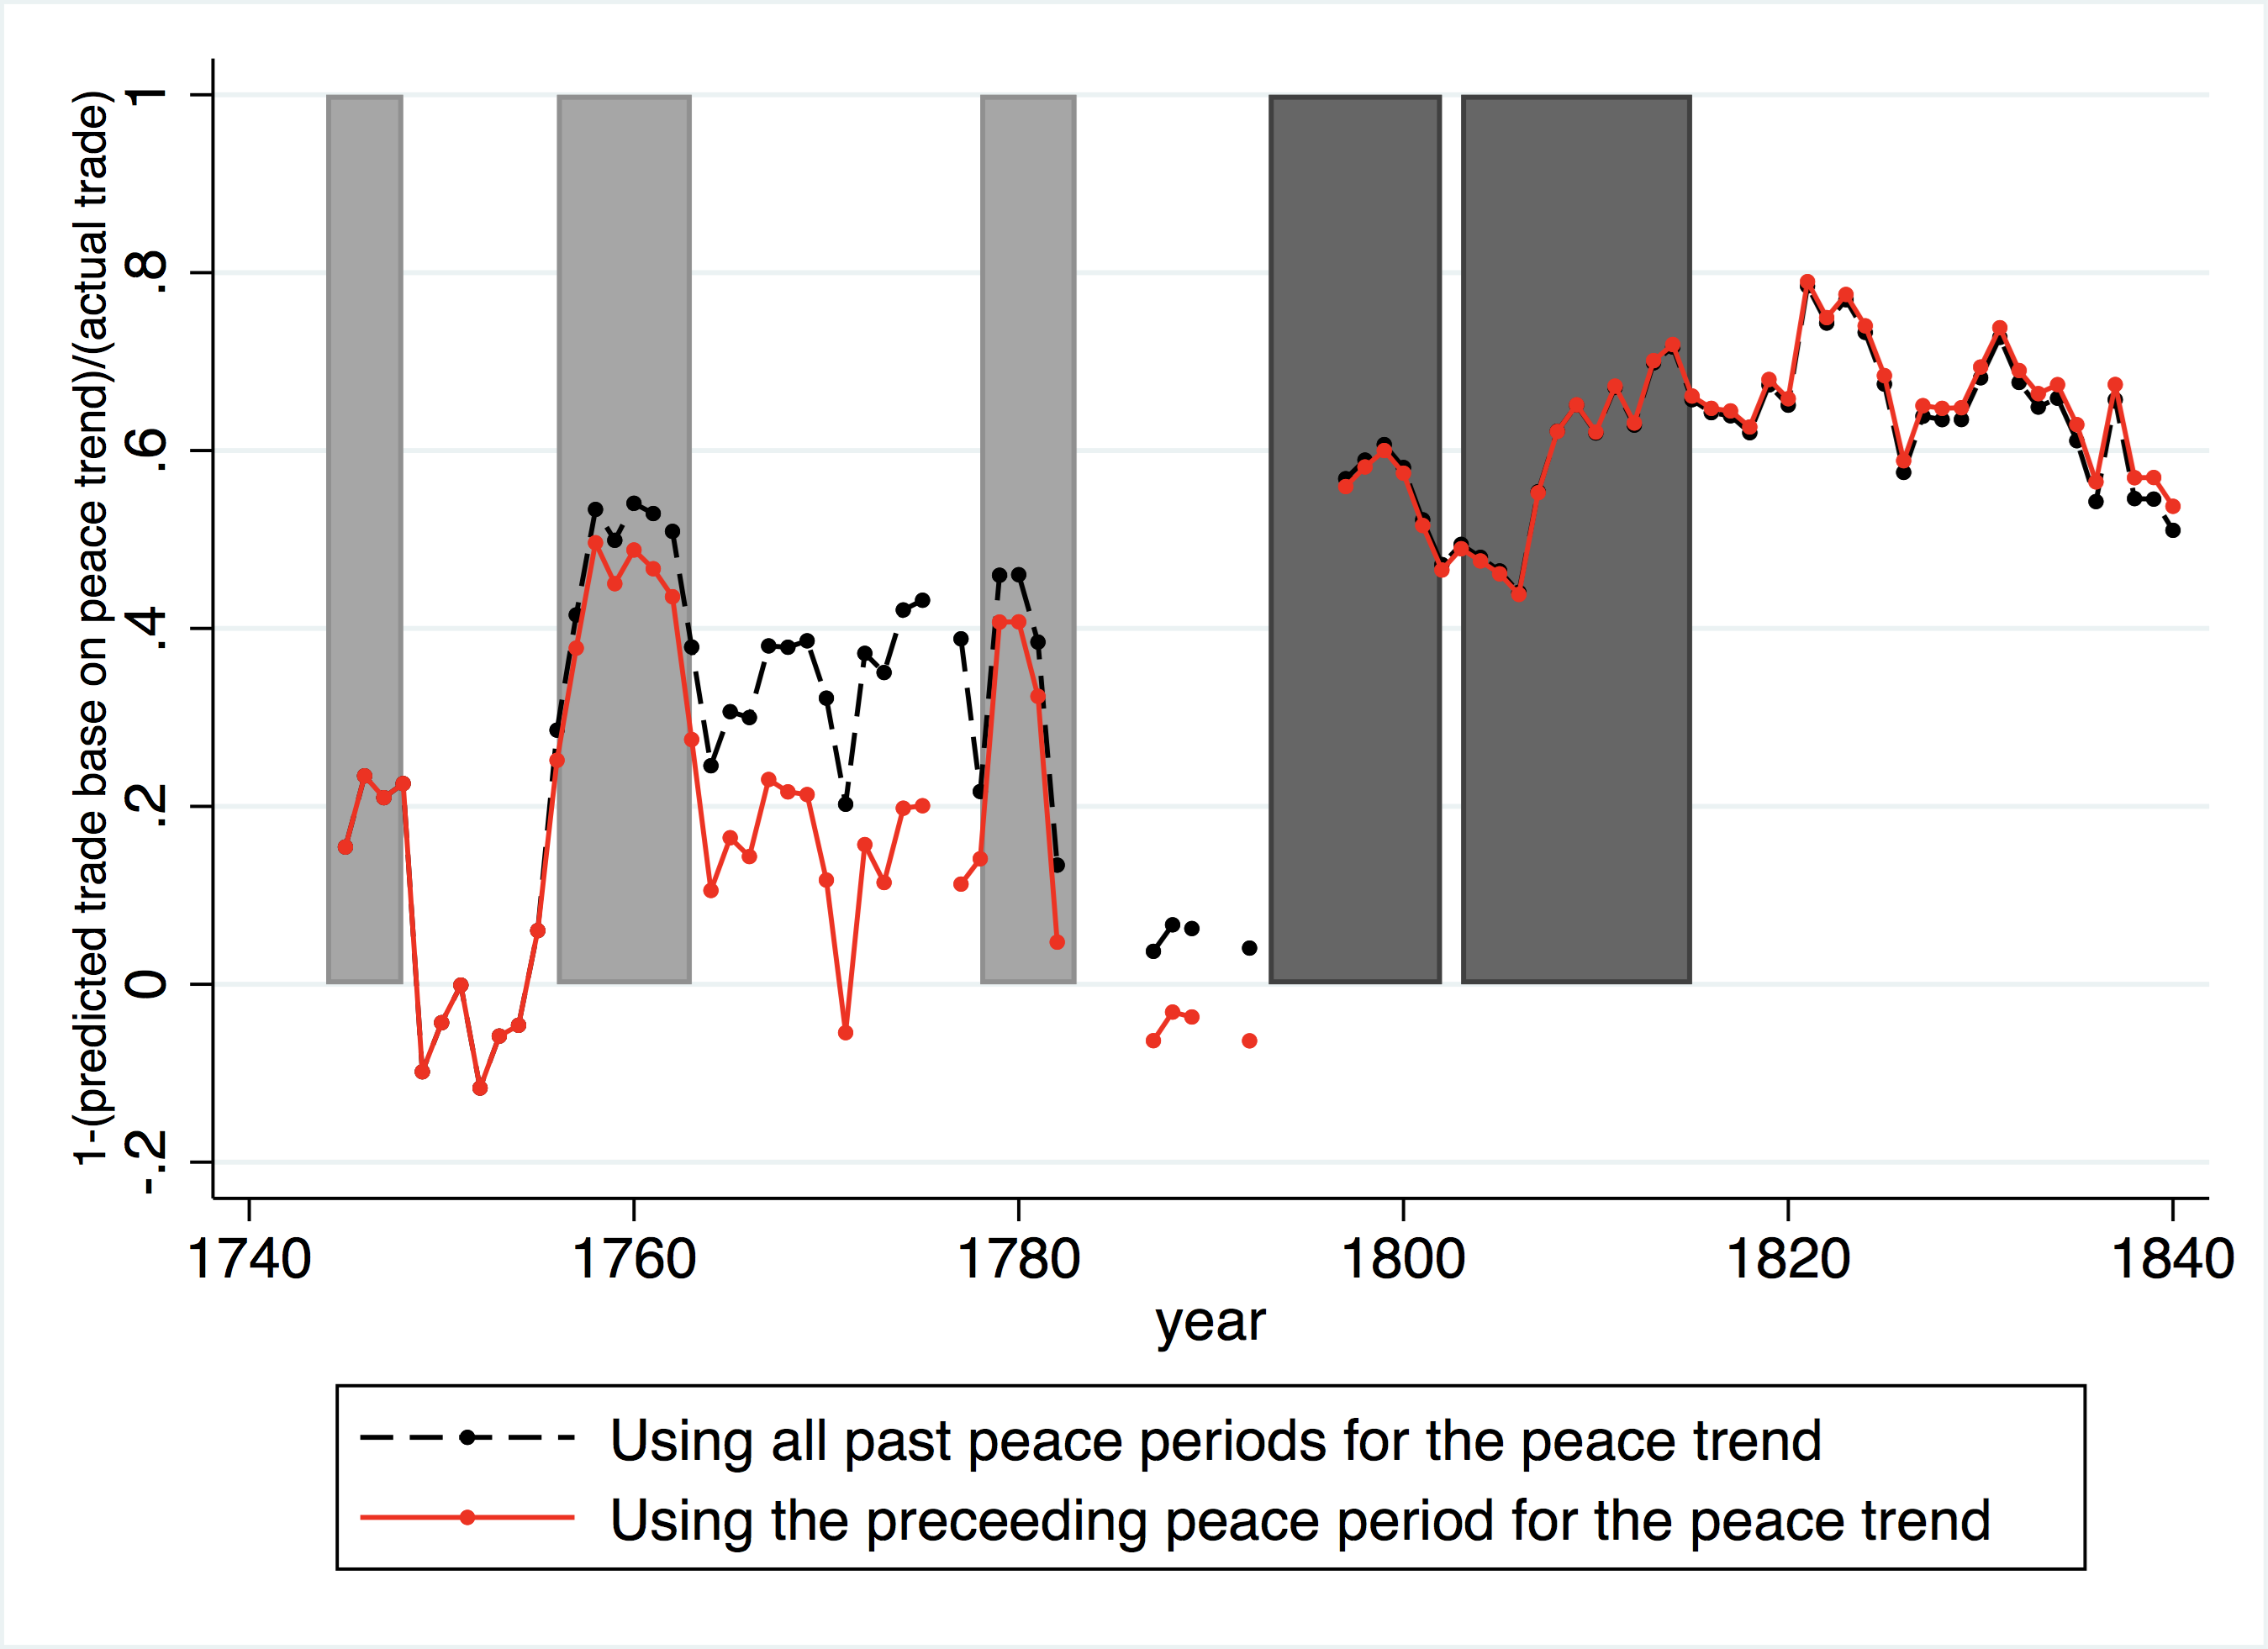
\includegraphics[scale=.425]{Annual_loss_function.png}
\caption{Mean Loss Function}
\label{mean_loss_function}
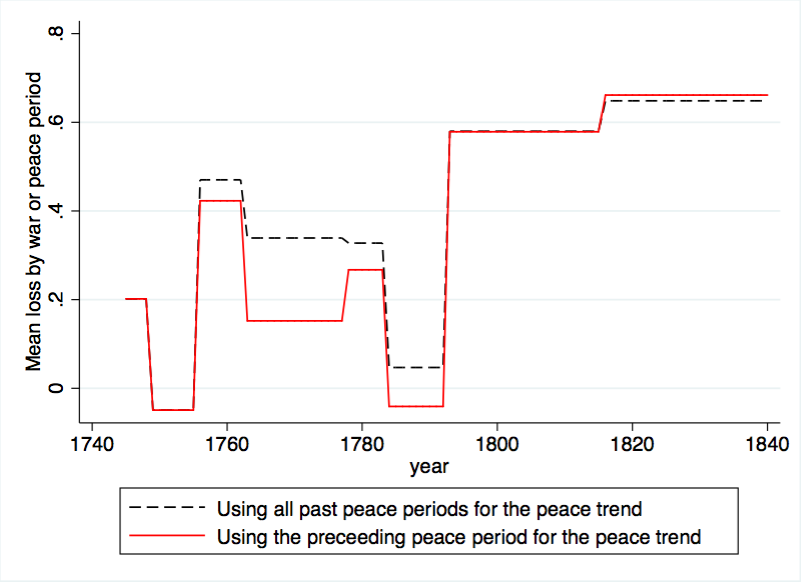
\includegraphics[scale=.4]{Mean_loss_function.png}
\end{figure}
\end{center}
\subsection{Explanatory variables}
We want to test the hypothesis that the most efficient strategy to curtail enemy's trade was to cut its commercial relations with neutral countries.
In order to do this, we run the following specification: 
\begin{equation*}
Loss = \beta_0 + \beta_1NavalSupremacy+ \beta_2ColonyLoss+ \beta_3NeutralRegulation
\end{equation*}
We use the loss function as a dependent variable, transformed from percentage to absolute value and then take the logs. \\
As explanatory variables we introduce several factors.
%NAVAL SUPREMACY
First, we use number of warships, grouped by belligerent/neutral status, as a proxy for naval supremacy. Figure \ref{naval_supremacy_ratios} reports the ratio of France over Great Britain, France and its allies versus Britain and its allies and France, its allies and neutral countries versus Britain and its allies.
Mostly, among neutral countries, we find Denmark, Hanseatic cities, United States and Russia.
The latter, however, occasionally was also allied with France (during Seven Years War for instance).
Ally countries were mostly colonies and, as mentioned, occasionally Russia.
We can observe here that the France-GB ratio is quite stable over the whole period, quite less so if we take into account allies and neutral.
The latter two ratios in fact, actually increase in the period of the Seven Years War and after, and also has some spikes during the Napoleonic Wars.
At least at first sight, this does not look related to the pattern of the loss function.
Intuitively, we would expect the loss to decrease as the ratio increases, therefore a positive relation.
\begin{center}
\begin{figure}[H]
\caption{Naval Supremacy Ratio}
\label{naval_supremacy_ratios}
\centering
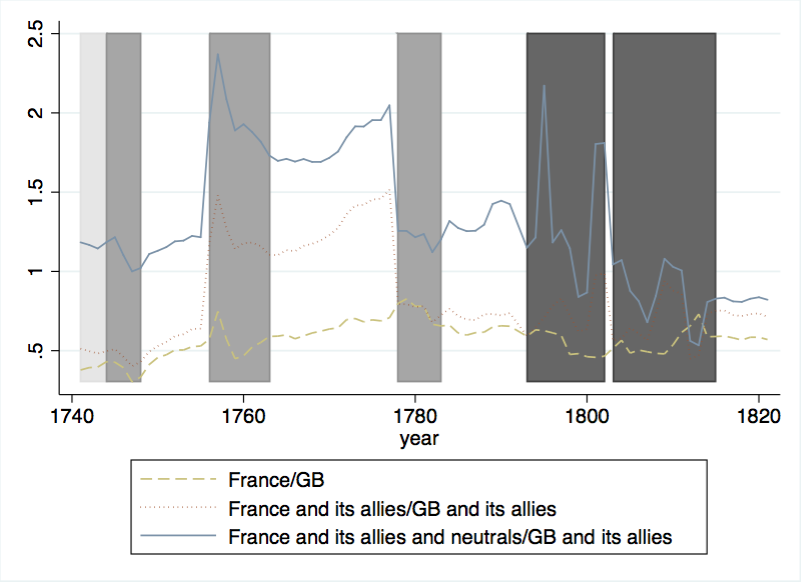
\includegraphics[scale=.51]{naval_supremacy_ratios.png}
\end{figure}
\end{center}
%COLONY LOSS MEASURE
Second, we include a colony loss measure.
At the time, the French empire owned several colonies in America, Asia and Africa.
Especially the American ones were a major source for production of sugar and coffee, which were widely imported and then re-exported by France to other European countries.
These territory, therefore, represented a valuable source for French trade, in particular St. Domingo, Guadeloupe and Martinique, which were major provider of sugar.
The former, which accounted for roughly 80\% of French imports in 1788 and was producing 60\% of total European coffee consumption, declared its independence in 1804 and separated from the French empire, thus depriving France of one of its main sources of colonial goods.
As a matter of fact, the revolt of the slaves in Haiti was a long and bloody episode and sugar production was lost well before independence was ultimately acquired.
This is easily visible in the graph, where the measure of colonial empire drops from 1 to just a little bit above 0.2 already in 1793.
In 1796, the measure increases again, as the revolt was partially under control and France was able to continue production and trade of sugar for a few years.
This only lasted until 1804, when ultimately Haiti became independent and France lost its main source of exports for sugar.
Guadeloupe was also important for its sugar production and was lost to the British between 1759 to 1763, as it is visible from the decrease of the index in the graphs, and between 1810 and 1816.
Finally, Martinique was controlled almost continuously by the British, from 1794-1815, to be traded back to France, after the Napoleonic Wars.
We have, therefore, created a weight variable, assigning to each colony a weight corresponding to its share of imports in 1788, for which we have data on single colony, and then interacted it with a dummy variable indicating whether that colony was under French possession in that specific year.
When France had all its colonies this variable equals 1, any time one colony is missing this variable equals 1 minus the share of imports of that particular colony.
For the specific case of St. Domingue, we coded the possession variable as 0 between 1793 and 1795, when the revolt started, and production was mostly destroyed or fields burnt.
For the period 1795 to 1804 we have coded it as 0.5, to account for the fact that the order was partly restored and a portion of the plantation were being cultivated normally, and only 1805 Haiti became independent and the production was lost completely.
Intuitively, we would expect a negative effect of this variable on the loss function; i.e. the more this measure increases (the closest it is to 1), the smaller the losses in trade on the French side.
Figure \ref{colony_loss} shows the evolution of the colony loss measure.
\begin{center}
\begin{figure}[H]
\caption{Measure of colonial empire}
\label{colony_loss}
\centering
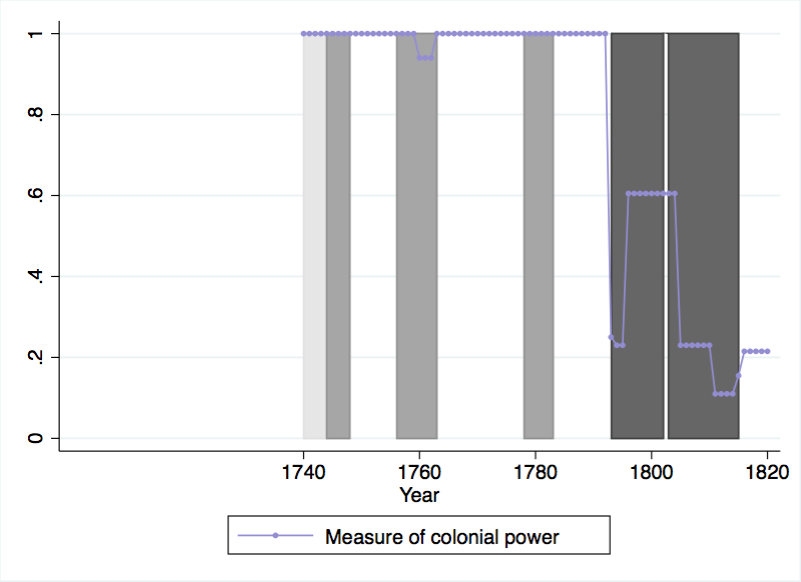
\includegraphics[scale=.51]{colony_loss.png}
\end{figure}
\end{center}
As we can see, for most of the eighteenth century, French empire encompassed most of its colonies, whereas after the French Revolution a substantial part of its empire was lost either to the British or because colonies obtained independence. \\
%CHRONOLOGY OF NEUTRAL COUNTRIES
Finally we introduce a categorical variable to measure the strictness of commercial policies versus neutral countries in wartime.
Initially, the only enemies were foes, while neutral countries were allowed to continue their trade with all other partners, despite an ongoing conflict.
This rule, however, had induced belligerent countries to exploit neutral ships for trading their own merchandises \citep{carriere1973negociants}.
For this reason, in 1756, during Seven Years War, the British decided to put an end to this practice and produced the \textit{Doctrine of Continuous Voyage}, which was forbidding neutrals, in time of war, to enjoy a trade from which they were barred in time of peace.
This prohibition was allowing the British to seize neutral shipping and had a considerable impact on French trade, which was heavily relying on Dutch ships to transport colonial goods.
It also created great discontent among neutral countries, which, however, were not able to enforce their rights efficiently until 1780, when, finally, Russia, Norway and Sweden created the \textit{League of Armed Neutrality}.
The latter allowed them to defend their interest at least for the time of the War of American Revolution.
This experiment however did not have a long lasting success and was finally put to an end in 1783 with the treaty of Paris, when Catherine of Russia renamed it the \textit{Armed Nullity}\footnote{The number of vessels Russia, Norway and Sweden owned combined were still less than the entire British navy, therefore this league was bound to be weak from the very beginning.} \citep{griffiths1971american}.
In 1793, with the outburst of the French Revolution and, subsequently, the Revolutionary Wars, most British goods were prohibited in France.
As a response, the British adopted a policy for blockading the coast of France and, subsequently, both countries took action against neutral shipping.
A year later, Denmark and Sweden attempted again to enforce their rights by creating a \textit{Second League of Armed Neutrality}, which was joined by Russia and Prussia in 1800.
No later than 1801, though, the British blockaded them (with the exception of Prussia) and bombed Copenhagen to end the League for good.
In 1806, things worsen even further for neutral countries, when Napoleon enacted the Berlin decree, which provided the basic structure of the Continental System.
The provisions of the Berlin Decree included: (1) prohibition of all trade with the British; (2) all British subjects in French-occupied areas were prisoners of war and their property was "fair prize"; (3) all trade in British goods was prohibited and all goods from England and her colonies were fair prize (and one-half their value was to be used to indemnify French merchants for losses to the British); and (4) no ships coming from the ports of Britain or its colonies would be permitted to use any port on the Continent \citep{davis2006naval}.
Britain responded to this policy with a related Order in Council, which required that neutral vessels call at a British port before proceeding to the continent, hitting at neutrals such as the United States, as well as France \citep{davis2006naval}.
The United States, were, at the time, the biggest neutral country whose trade was suffering because of the Blockade and, as a consequence, they attempted to fight back.
They first enacted, in 1807, an Embargo Act directed against trade with both France and Britain, which was followed by the Non-Intercourse Act of 1809, and finally, after failure of both provisions, by a war against Britain.
The United States had no better luck than France in the war, which was ultimately won by British, even if with considerable decline in trade for both sides.
The situation started to unravel only around 1810, when Russia pulled out of the Continental Blockade, pushing Napoleon to attempt an invasion, which ultimately led to his final defeat, but put an end to the Blockade System and to the threat for neutral trade.
Basing on these facts, we have created a categorical variable that can take three values; 0 if only enemy cargo were fair game, 1 if enemy cargo on neutral ships were fair game, 3 if any good from enemy territory  were fair game.
As a consequence, for this variable, we would expect a positive effect; the higher the value, the stricter the policy and the bigger the loss.
The table \ref{neutral_policy} reports the value of this variable overtime.
Table \ref{summary} reports a summary of all expected effects of the independent variables.
\begin{table}[H]
\centering
\caption{Measure of neutral policy}
\label{neutral_policy}
\begin{tabular}{ll}
\hline \hline
Period & Neutral policy variable  \\ \hline
1741-1755 & 0                  \\
1756-1779 & 1       \\
1780-1789 & 0                 \\
1797-1814 & 2                 \\
1815-1820 & 0                 \\
\hline 
\end{tabular}
\end{table}

\begin{table}[H]
\centering
\caption{Summary of expected effects}
\label{summary}
\begin{tabular}{ll}
\hline \hline
Explanatory Variable & Expected Effect  \\ \hline
Loss of colonies & \textbf{-}                  \\
Naval Supremacy & \textbf{-}                 \\
Treatment of neutral countries &       \textbf{+}      \\ \hline 
\end{tabular}
\end{table}



\iffalse
The unique database we are using allows us to do so in more details than it has been done so far.
In fact, we are not only doing it for aggregate trade for all countries but also distinguishing between neutral and foes and looking at a breakdown by products and sectors. \\
The first distinction is because we aim at uncovering the weight of neutral trade on global commerce in the eighteenth century.
The role of neutral has long been discussed and we aim to contribute to this debate.
The second is to observe variations in impact across products and sectors.
Products were traded from and to very different places, and it is legitimate to believe they might have been impacted differently.
For this reason we want to observe the effect of conflicts on specific products as well.\\
This latter task, however, was not an easy one.
The number of reported products is quite high and mostly they do not appear repeatedly (They either have different names or they are grouped together with different products).
For this reason we have chosen to use only the two main European products (Wine and Eau-de-vie) and the two main colonial products (Coffee and Sugar), which also represent the main share of French trade at the time, in value terms.
We have aggregated all the other products in one single category which we refer to as "Other".
As for the sectoral study, things were a bit easier, as we were able to classify all the products using the SITC classification.\\
Instead of looking at each war, one by one, we have made a distinction between the following two types of war: Mercantilist Wars (between 1744 and 1808) and Blockade Wars (from 1808 to 1820).
The former differs from the latter in that the political settings in second half of the eighteenth century were altered as a consequence of the French Revolution.
Therefore, we decided to make a distinction between wars before 1808, which were rather driven by economic interest, and the Continental Blockade, which, on the other hand, had more of a political goal.
%TECHNOLOGICAL CHANGE BEFORE AND AFTER BLOCKADE
Also, in that same period, an improvement in the British blockade strategy took place.
There were essentially two possible types of blockades \citep{rainerdevelopment}; the open and the closed blockade.
The former consisted of keeping the ships at port, but ready to sail, as soon as the enemy fleet left its harbour.
This technique was much less straining for men and ships, but less efficient when it came to blockading.
On the other hand, the closed blockade consisted of keeping the rival fleet blocked in its own port, impeding it from exiting.
This was much more of an efficient technique, however, the maintenance of both ships and men at sea for such a long time was a substantial issue.
By the end of eighteenth century, the British had implemented a very efficient system of resupply, in which supply ships delivered victuals to the fleet at sea, thus allowing it not to return at port regularly for supplies.
Also, they were being very careful to provide a balanced diet against scurvy, which passed from being a major issue for sails-men, to accounting for only 2 per cent of British naval patients between 1795 and 1800.
\citep{rodger2005command}.
On top of this, British had started to coat their ships with copper, to fight the issue of barnacles, oysters and the shipworm, which were seriously hindering the speed and the security of their vessels.
This dramatically reduced the possibility of avoid the blockade and allowed British to impede unwanted trade more efficiently.
Finally, we are more interested in the impact of wars in general, rather than each single war of the eighteenth century.
In the robustness section of this paper we also use two other possible classifications.
We do so both for imports and exports, running the following specifications: 
\begin{multline}\label{eq:1}
Flow_{t}=\exp\{\beta_0+\beta_1Status_jWar_k + \beta_2WarYearStatus_jWar_k+\beta_3Country_l +\beta_4YearCountry_l\}
\end{multline}
Where $Status_j$ is a dummy which indicates either foe or neutral, $War_k$ is another dummy which takes value 1 during the years of war, or is an indicator for which kind of war is taking place, $Year$ is the time trend and $Country_l$ and $YearCountry_l$ are respectively country fixed effects and year time trend.
This first specification provides information on the effects of war, or groups of war, depending on the situation of the country at stake (neutral of foes).
\begin{multline}\label{eq:2}
Flow_{t}=\exp\{\beta_0+\beta_1Status_jWar_k + \beta_2WarYearStatus_jWar_k+\beta_3Country_lProduct_i +\\ +\beta_4YearCountry_lProduct_i\}
\end{multline}
Equation \ref{eq:2} differs from equation \ref{eq:1} in that we have run on the database disaggregated by product and we have used country-product fixed effects and country-product time trend instead.
\begin{multline}\label{eq:3}
Flow_{t}=\exp\{\beta_0+\beta_1Status_jWar_k + \beta_2Country_lProduct_i+\beta_3YearCountry_lProduct_i\}
\end{multline}
Specification \ref{eq:3} allows us to look at effects of each group of war on the trade with allies and foes, by using product fixed effects and country-product time trend.
\begin{multline}\label{eq:4}
Flow_{t}=\exp\{\beta_0+\beta_1Product_iWar_k + \beta_2WarYearProduct_iWar_k+\beta_3Product_i +\\ +\beta_4YearProduct_i\}
\end{multline}
In equation \ref{eq:4} we are testing again the effects of kind of wars on products but by using product fixed effects and time trend, as opposed to country-product fixed effects and trends.
\begin{multline}\label{eq:5}
Flow_{t}=\exp\{\beta_0+\beta_1Product_iWar_k + \beta_2WarYearProduct_iWar_k+\beta_3Country_lProduct_i +\\ +\beta_4YearCountry_lProduct_i\}
\end{multline}
In this fifth specification $WarYearProduct$ is the time trend computed only over the war years and $War_k$ is interacted with $Product_i$, so we can observe the effect of the different kind of conflicts on the specific products.
\begin{multline}\label{eq:6}
Flow_{t}=\exp\{\beta_0+\beta_1Product_iWar_k + \beta_2Product_iCountry_l+\beta_3YearCountry_lProduct_i\}
\end{multline}
Finally, equation \ref{eq:6} provides an insight for the effects of groups of wars on specific products. \\
We start by using exports as explained variable and the five goods as \textit{products} (coffee, sugar, wine, eau-de-vie and others), in all the above mentioned six specifications.
Later we will repeat the analysis using imports and sectors.
Table \ref{table:export_class_war} reports the result of the first case where we have used a dummy just for peace or war, with no distinction on the kind of conflict.
\begin{table}
\begin{center}
\caption {Exports, Mercantilist Wars and Continental Blockade} 
\label{table:export_class_block}
\renewcommand{\arraystretch}{0.6}
{
\def\sym$\times$1{\ifmmode^{$\times$1}\else\(^{$\times$1}\)\fi}
\begin{tabular}{l*{6}{c}}
\hline\hline\\
                    &\multicolumn{1}{c}{(1)}&\multicolumn{1}{c}{(2)}&\multicolumn{1}{c}{(3)}&\multicolumn{1}{c}{(4)}&\multicolumn{1}{c}{(5)}&\multicolumn{1}{c}{(6)}\\
\hline\\
Allies$\times$Blockade&       0.227         &       0.195         &     -0.0252         &                     &                     &                     \\
                    &      (1.27)         &      (1.45)         &     (-0.24)         &                     &                     &                     \\
[1em]
Allies$\times$Mercantilist&      -0.130         &      -0.126         &     -0.0444         &                     &                     &                     \\
                    &     (-1.51)         &     (-1.55)         &     (-0.59)         &                     &                     &                     \\
[1em]
Foes$\times$Blockade&      -0.675** &      -0.676** &     -0.0201         &                     &                     &                     \\
                    &     (-2.71)         &     (-3.06)         &     (-0.17)         &                     &                     &                     \\
[1em]
Foes$\times$Mercantilist&      -0.463         &      -0.443         &      -0.560*  &                     &                     &                     \\
                    &     (-1.18)         &     (-1.27)         &     (-2.35)         &                     &                     &                     \\
[1em]
Neutral$\times$Blockade&      -1.403***&      -1.377** &      -0.586** &                     &                     &                     \\
                    &     (-3.35)         &     (-3.08)         &     (-2.99)         &                     &                     &                     \\
[1em]
Neutral$\times$Mercantilist&     -0.0809         &     -0.0265         &      -0.164*  &                     &                     &                     \\
                    &     (-0.66)         &     (-0.25)         &     (-2.02)         &                     &                     &                     \\
[1em]
Coffee$\times$Blockade&                     &                     &                     &      -2.966** &      -2.970***&      -2.891***\\
                    &                     &                     &                     &     (-3.25)         &     (-3.89)         &     (-4.93)         \\
[1em]
Coffee$\times$Mercantilist&                     &                     &                     &      -0.314         &      -0.305         &      -0.388         \\
                    &                     &                     &                     &     (-0.93)         &     (-1.20)         &     (-1.14)         \\
[1em]
Eau de vie$\times$Blockade&                     &                     &                     &       0.398         &       26.42         &       28.80         \\
                    &                     &                     &                     &      (1.43)         &      (0.94)         &      (1.03)         \\
[1em]
Eau de vie$\times$Mercantilist&                     &                     &                     &      -0.367         &       25.90         &       28.61         \\
                    &                     &                     &                     &     (-1.08)         &      (0.92)         &      (1.02)         \\
[1em]
Other$\times$Blockade&                     &                     &                     &     -0.0599         &      -35.28         &      -35.98         \\
                    &                     &                     &                     &     (-0.79)         &     (-1.05)         &     (-1.07)         \\
[1em]
Other$\times$Mercantilist&                     &                     &                     &      -0.177         &      -35.37         &      -36.12         \\
                    &                     &                     &                     &     (-1.49)         &     (-1.05)         &     (-1.07)         \\
[1em]
Sugar$\times$Blockade&                     &                     &                     &      -3.813***&       122.7** &       126.3** \\
                    &                     &                     &                     &     (-4.07)         &      (2.95)         &      (2.97)         \\
[1em]
Sugar$\times$Mercantilist&                     &                     &                     &      -0.151         &       126.5** &       130.0** \\
                    &                     &                     &                     &     (-0.51)         &      (3.05)         &      (3.06)         \\
[1em]
Wine$\times$Blockade&                     &                     &                     &      -0.189         &       22.18         &       21.40         \\
                    &                     &                     &                     &     (-0.91)         &      (0.81)         &      (0.78)         \\
[1em]
Wine$\times$Mercantilist&                     &                     &                     &      -0.241         &       22.26         &       21.30         \\
                    &                     &                     &                     &     (-1.32)         &      (0.81)         &      (0.78)         \\
[1em]
Constant            &      -20.17***&      -63.73***&      -64.62***&      -0.320         &      -75.42***&      -75.36***\\
                    &     (-4.29)         &     (-3.55)         &     (-3.64)         &     (-0.03)         &     (-3.90)         &     (-3.88)         \\
\hline\\
Observations        &        1010         &        5050         &        5050         &         445         &        5050         &        5050         \\
\hline\hline
\multicolumn{7}{l}{\footnotesize \textit{t} statistics in parentheses}\\
\multicolumn{7}{l}{\footnotesize * \(p<0.05\), ** \(p<0.01\), *** \(p<0.001\)}\\
\end{tabular}
}

\end{center}
\end{table}
\begin{table}
\begin{center}
\caption {Imports, Mercantilist Wars and Continental Blockade} 
\label{table:import_class_block}
\renewcommand{\arraystretch}{0.6}
{
\def\sym$\times$1{\ifmmode^{$\times$1}\else\(^{$\times$1}\)\fi}
\begin{tabular}{l*{6}{c}}
\hline\hline
                    &\multicolumn{1}{c}{(1)}&\multicolumn{1}{c}{(2)}&\multicolumn{1}{c}{(3)}&\multicolumn{1}{c}{(4)}&\multicolumn{1}{c}{(5)}&\multicolumn{1}{c}{(6)}\\
\hline
Allies$\times$Blockade&     -0.0395         &      0.0222         &      -0.265*  &                     &                     &                     \\
                    &     (-0.18)         &      (0.18)         &     (-2.57)         &                     &                     &                     \\
[1em]
Allies$\times$Mercantilist&      -0.183         &      -0.154         &      -0.135*  &                     &                     &                     \\
                    &     (-1.55)         &     (-1.81)         &     (-2.19)         &                     &                     &                     \\
[1em]
Foes$\times$Blockade&      -0.561         &      -0.379         &      -0.173*  &                     &                     &                     \\
                    &     (-1.86)         &     (-1.89)         &     (-1.96)         &                     &                     &                     \\
[1em]
Foes$\times$Mercantilist&      -0.497         &      -0.478         &      -0.642***&                     &                     &                     \\
                    &     (-1.55)         &     (-1.75)         &     (-3.42)         &                     &                     &                     \\
[1em]
Neutral$\times$Blockade&      -1.146***&      -1.115***&      -0.737***&                     &                     &                     \\
                    &     (-3.42)         &     (-3.90)         &     (-5.36)         &                     &                     &                     \\
[1em]
Neutral$\times$Mercantilist&     -0.0261         &      0.0177         &     -0.0625         &                     &                     &                     \\
                    &     (-0.26)         &      (0.21)         &     (-1.01)         &                     &                     &                     \\
[1em]
Coffee$\times$Blockade&                     &                     &                     &      -2.135***&      -2.007***&      -2.061***\\
                    &                     &                     &                     &     (-5.93)         &     (-4.19)         &     (-6.12)         \\
[1em]
Coffee$\times$Mercantilist&                     &                     &                     &      -0.597*  &      -0.554*  &      -0.498*  \\
                    &                     &                     &                     &     (-2.09)         &     (-2.13)         &     (-2.09)         \\
[1em]
Eau de vie$\times$Blockade&                     &                     &                     &       0.183         &       41.31         &       43.52         \\
                    &                     &                     &                     &      (0.70)         &      (1.61)         &      (1.72)         \\
[1em]
Eau de vie$\times$Mercantilist&                     &                     &                     &      -0.350         &       40.89         &       43.50         \\
                    &                     &                     &                     &     (-1.17)         &      (1.60)         &      (1.73)         \\
[1em]
Other$\times$Blockade&                     &                     &                     &      -0.150*  &       19.45         &       19.71         \\
                    &                     &                     &                     &     (-2.18)         &      (1.04)         &      (1.06)         \\
[1em]
Other$\times$Mercantilist&                     &                     &                     &      -0.101         &       19.47         &       19.74         \\
                    &                     &                     &                     &     (-1.19)         &      (1.05)         &      (1.06)         \\
[1em]
Sugar$\times$Blockade&                     &                     &                     &      -1.371         &       68.46** &       68.73** \\
                    &                     &                     &                     &     (-1.54)         &      (2.76)         &      (2.77)         \\
[1em]
Sugar$\times$Mercantilist&                     &                     &                     &      -0.329         &       69.37** &       69.84** \\
                    &                     &                     &                     &     (-1.19)         &      (2.80)         &      (2.82)         \\
[1em]
Wine$\times$Blockade&                     &                     &                     &      -0.210         &       39.24         &       38.63         \\
                    &                     &                     &                     &     (-1.03)         &      (1.53)         &      (1.50)         \\
[1em]
Wine$\times$Mercantilist&                     &                     &                     &      -0.236         &       39.29         &       38.54         \\
                    &                     &                     &                     &     (-1.33)         &      (1.53)         &      (1.50)         \\
[1em]
Constant            &      -27.31***&      -84.87***&      -85.02***&      -17.63*  &      -94.32***&      -94.32***\\
                    &     (-5.78)         &     (-7.84)         &     (-7.90)         &     (-2.28)         &     (-7.50)         &     (-7.53)         \\
\hline
Observations        &        1010         &        9792         &        9792         &         445         &        9792         &        9792         \\
\hline\hline
\multicolumn{7}{l}{\footnotesize \textit{t} statistics in parentheses}\\
\multicolumn{7}{l}{\footnotesize * \(p<0.05\), ** \(p<0.01\), *** \(p<0.001\)}\\
\end{tabular}
}

\end{center}
\end{table}
The six regressions in table \ref{table:export_class_block} report the results.
For this set of analysis we have split the conflicts again in two groups, but this time distinguishing between any war (1717-1787) and Continental Blockade (from 1808).
In this setting we notice a difference with respect to the pattern seen before.
Adversaries see a decrease in trade only according to specification \ref{eq:1} and \ref{eq:2} but not to specification \ref{eq:3}, however, neutral during the Blockade years, experience a very substantial decrease in trade.
This would suggest that, whereas wartime was mostly damaging for trade towards enemies, the continental Blockade period, during which overall French trade lost to British, had damaged neutral countries, rather than Britain, which was the original target.
It is quite likely, therefore, that before the Blockade had taken place, war did not represent such a danger for merchants, who were able to continue their trade through other channels, i.e. "neutral cargo" policy.
On the other had, during Continental Blockade years, which were meant to damage British trade, regulation on neutral cargo had become much stricter, and this is where we observe a collapse in trade with neutral countries and a massive decrease in overall trade.
As a consequence, we are prone to avail \cite{riley_seven_1986}'s theory on the small effects of wars on commerce, at least until the twentieth century, thanks to the ability of merchants to exploit neutral ships and workaround of wartime restrictions.\\
We repeat now all the three different analysis above on imports and we report them in tables \ref{table:import_class_war} to \ref{table:import_class_block}.
From table \ref{table:import_class_war} we observe a very similar pattern with respect to the previous analysis.
Wars in general are disruptive for trade towards foes, however there is no coherent evidence that neutral and allies were strongly affected at all.
By looking at table \ref{table:import_class_merc} we observe, again, that imports from foes were strongly affected by Revolutionary and Napoleonic conflicts.
Differently from before, there is a negative effect for allies, which was not the case for exports, and also a mild but significant impact for neutral countries during Mercantilist wars.
Product-wise the situation is again similar, as we observe strong decrease in import of sugar but again an increase in import of eau-de-vie.
As for table \ref{table:import_class_block}, once more it is evident the massive effect of the blockade on neutral trade.
Not only exports but also imports from neutral countries were seriously damaged by the Blockade, way less so than imports from enemies.
This goes once more in the direction of explaining the fall in trade of aggregate trade in the first half of the nineteenth century in France. \\

\fi
%The figures below give a more visual picture of the trend of the different products.
As for wine and eau-de-vie, war do not seem to have a great impact on their trend.
As for coffee and sugar, on the other hand, wars seem to be diminishing trade, however, given the big fluctuations all throughout, we cannot for sure distinguish between the effects of conflicts and the very variable pattern of trade.
%\begin{figure}[H]
%\begin{center}
%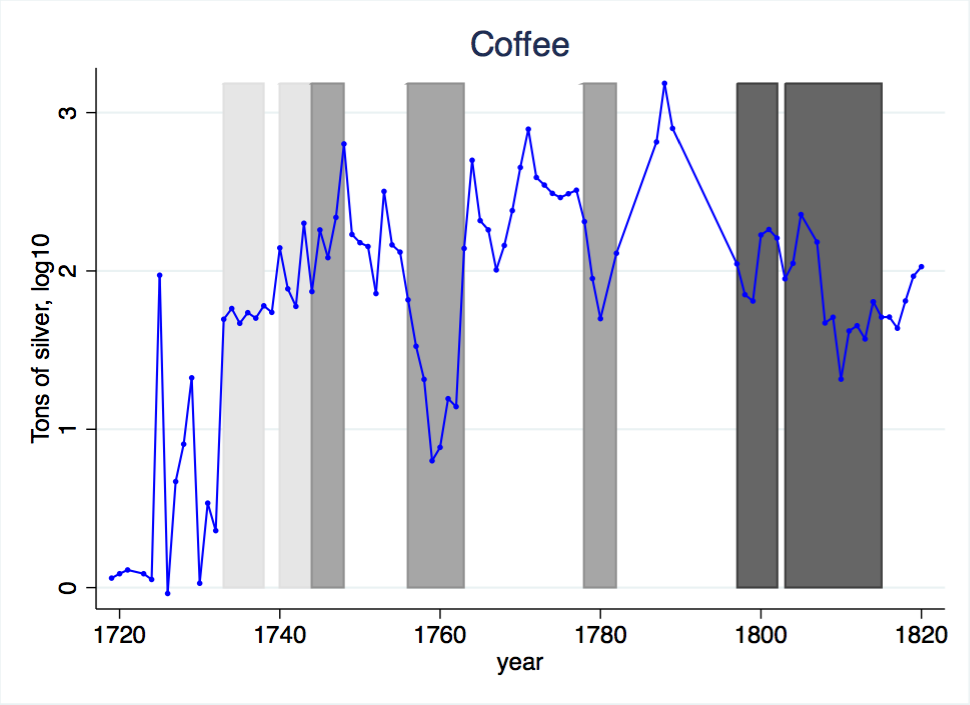
\includegraphics[scale=.25]{class1_trend}
%\hfil 
%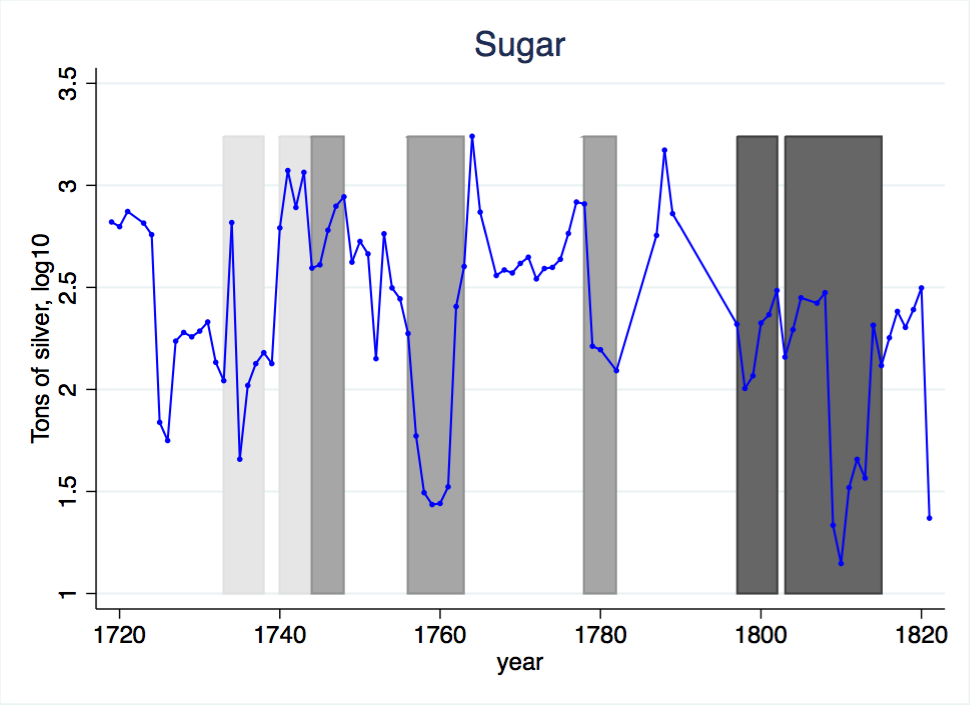
\includegraphics[scale=.25]{class3_trend}
%\vspace*{.7em}
%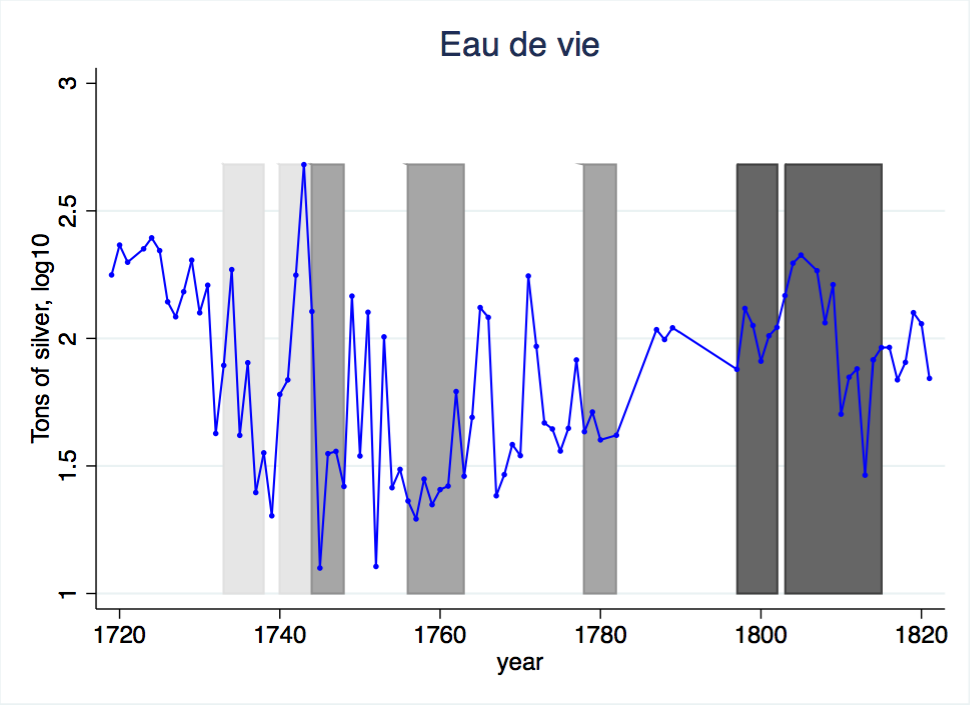
\includegraphics[scale=.25]{class2_trend}
%\hfil 
%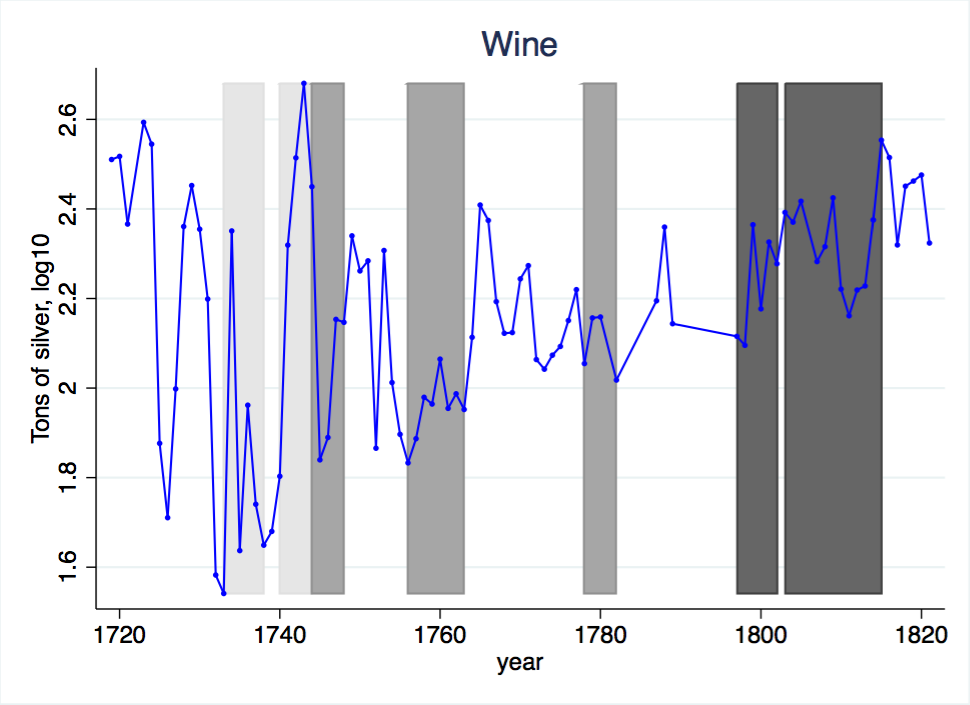
\includegraphics[scale=.25]{class4_trend}
%\end{center}
%\end{figure}

\iffalse
\subsection{War lags}
In line with this reasoning, we turned next to analyse and compare war lags in the Hamburg case and general case.
we run two regressions with and without product differentiation and for all wars together and a dummy for each war: 
\begin{multline}
\ln(exports_{i,t})=\beta_0+\beta_1country_i+\beta_2country_iyear+\beta_3adversaries_i+\beta_4neutral_i+\\+\beta_5adversary_ilag+\beta_6neutral_ilag+\beta_8allies_ilag
\end{multline}
\begin{multline}
\ln(exports_{i,t})=\beta_0+\beta_1country_i+\beta_2country_iyear+\beta_3product_{i,j}+\beta_4product_jyear+\\+\beta_5product_jadversary+ \beta_6product_jneutral+\beta_7product_jadversary_ilag+\beta_8neutral_ilag+\beta_9allies_ilag
\end{multline}

Results are quite in line with those seen in the Hamburg series.
There is no post war negative coefficient, but on the contrary, trade increases by 40\% and 47\% in the first and second year after the war.
Starting from the third year this effect decreases and coefficients are still positive but smaller. \\
Product-wise there is evidence of positive post war effects for all the products but in particular European products increase stably for the first four years after the war.
War by war, we notice an interesting pattern after Seven Years War; exports of European goods increases as for the general case, but here we see that trade of sugar as well expands right after the war (+62\%).
This is quite an interesting result given that sugar was, with coffee, the product which suffered the most during this conflict.
In sum, we can say that, as for the case of Hamburg, there is no clear evidence of war lags, for sure not 10 years lag as claimed by Glick and Taylor (2005).
Trade was extremely adaptive to conflicts in eighteenth century and neutral countries did not seem to suffer strong consequences.
we have also run the regression checking for pre war effects.
Results are positive but very small in size for the general case, except for the case of allies countries, which has larger and more significant coefficients.
The war-by-war case (considered all in one regression) is also not very meaningful; coefficients for Seven Years War are negative whereas those for American Revolutionary War are positive.
In terms of difference between products, the results are again not very interesting.
There is no stable pattern for pre war effect, except for coffee, which always shows an increase for all the four years preceding the war.
However this might be just due to the increasing trend shown by coffee, disregarding the effects of wars.
Overall, for neutral countries the compensation effect is more likely as a post war phenomenon rather than a pre war one, again as noted for the case of Hamburg.
\fi

\iffalse
\section{Robustness}
We have re-run our analysis using two other possible grouping of wars.
First considering all wars together (i.e. one dummy that takes value 1 whenever there is an ongoing conflict) and then by  Mercantilist wars (Polish and Austrian Succession, Seven Years War, American Revolutionary war) and Napoleonic and Revolutionary wars.
Table \ref{table:export_class_war} reports the result of the first case where we have used a dummy just for peace or war, with no distinction on the kind of conflict.
\begin{table}
\begin{center}
\caption {Exports, for all wars together} 
\label{table:export_class_war}
\renewcommand{\arraystretch}{0.6}
{
\def\sym$\times$1{\ifmmode^{$\times$1}\else\(^{$\times$1}\)\fi}
\begin{tabular}{l*{6}{c}}
\hline\hline
                    &\multicolumn{1}{c}{(1)}&\multicolumn{1}{c}{(2)}&\multicolumn{1}{c}{(3)}&\multicolumn{1}{c}{(4)}&\multicolumn{1}{c}{(5)}&\multicolumn{1}{c}{(6)}\\
\hline
Allies$\times$War&     -0.0800         &     -0.0691         &     -0.0619         &                     &                     &                     \\
                    &     (-0.92)         &     (-0.85)         &     (-0.91)         &                     &                     &                     \\
[1em]
Foes$\times$War&      -0.768*  &      -0.735*  &      -0.319*  &                     &                     &                     \\
                    &     (-2.20)         &     (-2.53)         &     (-2.27)         &                     &                     &                     \\
[1em]
Neutral$\times$War&      -0.114         &     -0.0480         &      -0.208** &                     &                     &                     \\
                    &     (-0.92)         &     (-0.46)         &     (-2.64)         &                     &                     &                     \\
[1em]
Coffee$\times$War&                     &                     &                     &      -0.116         &      -0.106         &      -0.594         \\
                    &                     &                     &                     &     (-0.31)         &     (-0.38)         &     (-1.57)         \\
[1em]
Eau-de-vie$\times$War&                     &                     &                     &      -0.396         &       21.29         &       16.41         \\
                    &                     &                     &                     &     (-1.35)         &      (0.79)         &      (0.62)         \\
[1em]
Other$\times$War&                     &                     &                     &      -0.218*  &      -40.06         &      -46.26         \\
                    &                     &                     &                     &     (-1.98)         &     (-1.22)         &     (-1.44)         \\
[1em]
Sugar$\times$War&                     &                     &                     &     -0.0190         &       132.0***&       147.4***\\
                    &                     &                     &                     &     (-0.06)         &      (3.30)         &      (3.61)         \\
[1em]
Wine$\times$War&                     &                     &                     &      -0.357*  &       16.57         &       10.72         \\
                    &                     &                     &                     &     (-2.15)         &      (0.62)         &      (0.41)         \\
[1em]
Constant            &      -20.79***&      -64.20***&      -65.73***&       1.256         &      -71.81***&      -67.07***\\
                    &     (-4.28)         &     (-3.62)         &     (-3.68)         &      (0.12)         &     (-3.93)         &     (-3.85)         \\
\hline
Observations        &        1010         &        5050         &        5050         &         445         &        5050         &        5050         \\
\hline\hline
\multicolumn{7}{l}{\footnotesize \textit{t} statistics in parentheses}\\
\multicolumn{7}{l}{\footnotesize * \(p<0.05\), ** \(p<0.01\), *** \(p<0.001\)}\\
\end{tabular}
}

\end{center}
\end{table}
From table \ref{table:export_class_war}, where we only consider wars interacted with war status and products, we can observe that the only consistently significant effect is the negative impact of war on trade with adversary countries.
For specifications \ref{eq:1} to \ref{eq:3} we can see a significant negative impact on the trade of France with foes.
On the other hand, if we look at the breakdown by product, in equations \ref{eq:4} to \ref{eq:6}, we observe that none of them is hit particularly by wars.
This would suggest that, despite the disruptive effects of conflicts on trade with enemies, the commercial exchange with allies and in particular with neutral could compensate for this loss.\\
Table \ref{table:export_class_merc} reports results for the six specifications run distinguishing between Mercantilist wars, i.e. wars between 1733 and 1782, and Napoleonic and Revolutionary Wars, from 1797 onwards.
Once more, we observe that across the three different specifications, there is no coherent effects of war on exports.
In fact, even if we observe a negative and significant effect for specifications \ref{eq:1} and \ref{eq:2} of Mercantilist Wars on exports to allies, this effect becomes small and insignificant in specification \ref{eq:3}, just by disregarding war-years time trends.
The only coefficient which is robust to all three specification is, again, effects of conflicts on trade with foes, more specifically in the case of Revolutionary and Mercantilist Wars.
This suggests that the effects of wars observed in table \ref{table:export_class_war} is probably driven by the fall in commerce during Napoleonic Wars.
Results for the effects on single products also yields further insights with respect to the previous table.
First of all we observe that coffee is subject to a massive decrease during Revolutionary and  Napoleonic Wars, regardless of the specification at stake.
On the other hand, wine and eau-de-vie see an increase in export during this second conflict.
This would actually suggests that war, in general, was not a major source of disruption in trade, for sure not Mercantilist War, and that decrease in exports was mostly due to decrease in the export of certain goods, whereas other goods, in war-time, actually experienced an increase in trade.\\
We repeat now all the two different analysis above on imports and we report them in tables \ref{table:import_class_war} and \ref{table:import_class_merc}.
From table \ref{table:import_class_war} we observe a very similar pattern with respect to the previous analysis.
Wars in general are disruptive for trade towards foes, however there is no coherent evidence that neutral and allies were strongly affected at all.
By looking at table \ref{table:import_class_merc} we observe, again, that imports from foes were strongly affected by Revolutionary and Napoleonic conflicts.
Differently from before, there is a negative effect for allies, which was not the case for exports, and also a mild but significant impact for neutral countries during Mercantilist wars.
This goes once more in the direction of explaining the fall in trade of aggregate trade in the first half of the nineteenth century in France.
\begin{table}
\begin{center}
\caption {Exports, distinguishing between Mercantilist War and Napoleonic and Revolutionary Wars} \label{table:export_class_merc}
\renewcommand{\arraystretch}{0.6}
{
\def\sym$\times$1{\ifmmode^{$\times$1}\else\(^{$\times$1}\)\fi}
\begin{tabular}{l*{6}{c}}
\hline\hline\\
                    &\multicolumn{1}{c}{(1)}&\multicolumn{1}{c}{(2)}&\multicolumn{1}{c}{(3)}&\multicolumn{1}{c}{(4)}&\multicolumn{1}{c}{(5)}&\multicolumn{1}{c}{(6)}\\
                    
\hline\\
Allies$\times$Mercantilis&      -0.315** &      -0.327***&      -0.107         &                     &                     &                     \\
                    &     (-3.08)         &     (-3.29)         &     (-0.86)         &                     &                     &                     \\
[1em]
Allies$\times$R\&N &     -0.0927         &      -0.194         &      -0.314** &                     &                     &                     \\
                    &     (-0.68)         &     (-1.55)         &     (-3.04)         &                     &                     &                     \\
[1em]
Foes$\times$Mercantilist&      -0.570         &      -0.560         &      -0.351         &                     &                     &                     \\
                    &     (-1.25)         &     (-1.36)         &     (-1.48)         &                     &                     &                     \\
[1em]
Foes$\times$R\&N &      -2.234***&      -2.270***&      -0.571***&                     &                     &                     \\
                    &     (-4.98)         &     (-6.25)         &     (-3.56)         &                     &                     &                     \\
[1em]
Neutral$\times$Mercantilist&      -0.165         &      -0.129         &      -0.250** &                     &                     &                     \\
                    &     (-1.15)         &     (-1.01)         &     (-2.61)         &                     &                     &                     \\
[1em]
Neutral$\times$R\&N &     -0.0662         &      -0.138         &      -0.528***&                     &                     &                     \\
                    &     (-0.35)         &     (-0.74)         &     (-3.78)         &                     &                     &                     \\
[1em]
Coffee$\times$Mercantilist&                     &                     &                     &      -0.599         &      -0.592*  &      -0.313         \\
                    &                     &                     &                     &     (-1.92)         &     (-2.43)         &     (-1.00)         \\
[1em]
Coffee$\times$R\&N &                     &                     &                     &      -4.908***&      -5.349***&      -5.135***\\
                    &                     &                     &                     &     (-7.35)         &     (-8.00)         &    (-11.88)         \\
[1em]
Eau de vie$\times$Mercantilist&                     &                     &                     &      -0.768         &       247.3***&       239.1***\\
                    &                     &                     &                     &     (-1.87)         &      (5.48)         &      (5.75)         \\
[1em]
Eau de vie$\times$R\&N &                     &                     &                     &       1.495***&       249.1***&       240.7***\\
                    &                     &                     &                     &      (4.85)         &      (5.51)         &      (5.78)         \\
[1em]
Other$\times$Mercantilist&                     &                     &                     &      -0.253         &       136.0** &       132.8** \\
                    &                     &                     &                     &     (-1.44)         &      (2.79)         &      (2.93)         \\
[1em]
Other$\times$R\&N &                     &                     &                     &    -0.00538         &       136.2** &       132.9** \\
                    &                     &                     &                     &     (-0.04)         &      (2.79)         &      (2.93)         \\
[1em]
Sugar$\times$Mercantilist&                     &                     &                     &      -0.279         &       108.0         &       101.2         \\
                    &                     &                     &                     &     (-0.99)         &      (1.95)         &      (1.93)         \\
[1em]
Sugar$\times$R\&N &                     &                     &                     &      -3.593***&       104.2         &       97.27         \\
                    &                     &                     &                     &     (-6.62)         &      (1.88)         &      (1.85)         \\
[1em]
Wine$\times$Mercantilist&                     &                     &                     &      -0.242         &       204.6***&       200.5***\\
                    &                     &                     &                     &     (-0.99)         &      (4.62)         &      (4.93)         \\
[1em]
Wine$\times$R\&N &                     &                     &                     &       0.549** &       204.9***&       200.9***\\
                    &                     &                     &                     &      (2.89)         &      (4.63)         &      (4.94)         \\
[1em]
Constant            &      -24.92***&      -73.86***&      -76.01***&      -52.71***&      -256.0***&      -252.5***\\
                    &     (-4.56)         &     (-3.91)         &     (-4.03)         &     (-5.23)         &     (-6.44)         &     (-7.07)         \\
\hline\\
Observations        &        1010         &        5050         &        5050         &         445         &        5050         &        5050         \\
\hline\hline
\multicolumn{7}{l}{\footnotesize \textit{t} statistics in parentheses}\\
\multicolumn{7}{l}{\footnotesize * \(p<0.05\), ** \(p<0.01\), *** \(p<0.001\)}\\
\end{tabular}
}

\end{center}
\end{table}
\begin{table}
\begin{center}
\caption {Imports, for all wars together} 
\label{table:import_class_war}
\renewcommand{\arraystretch}{0.6}
{
\def\sym$\times$1{\ifmmode^{$\times$1}\else\(^{$\times$1}\)\fi}
\begin{tabular}{l*{6}{c}}
\hline\hline
                    &\multicolumn{1}{c}{(1)}&\multicolumn{1}{c}{(2)}&\multicolumn{1}{c}{(3)}&\multicolumn{1}{c}{(4)}&\multicolumn{1}{c}{(5)}&\multicolumn{1}{c}{(6)}\\
\hline
Allies$\times$War   &      -0.135         &     -0.0828         &      -0.180** &                     &                     &                     \\
                    &     (-1.23)         &     (-1.09)         &     (-3.03)         &                     &                     &                     \\
[1em]
Foes$\times$War    &      -0.784** &      -0.696** &      -0.399***&                     &                     &                     \\
                    &     (-2.77)         &     (-3.17)         &     (-3.95)         &                     &                     &                     \\
[1em]
Neutral$\times$War&      0.0137         &      0.0638         &      -0.130*  &                     &                     &                     \\
                    &      (0.14)         &      (0.81)         &     (-2.16)         &                     &                     &                     \\
[1em]
Coffee$\times$War &                     &                     &                     &      -0.410         &      -0.325         &      -0.781** \\
                    &                     &                     &                     &     (-1.39)         &     (-1.35)         &     (-3.02)         \\
[1em]
Eau de vie$\times$War&                     &                     &                     &      -0.344         &       38.10         &       35.01         \\
                    &                     &                     &                     &     (-1.33)         &      (1.56)         &      (1.44)         \\
[1em]
Other$\times$War  &                     &                     &                     &      -0.121         &       15.39         &       12.14         \\
                    &                     &                     &                     &     (-1.52)         &      (0.86)         &      (0.69)         \\
[1em]
Sugar$\times$War  &                     &                     &                     &      -0.248         &       70.97** &       77.36***\\
                    &                     &                     &                     &     (-0.97)         &      (2.97)         &      (3.41)         \\
[1em]
Wine$\times$War   &                     &                     &                     &      -0.347*  &       33.80         &       28.32         \\
                    &                     &                     &                     &     (-2.14)         &      (1.35)         &      (1.16)         \\
[1em]
Constant            &      -27.66***&      -84.79***&      -84.91***&      -16.36*  &      -90.47***&      -86.15***\\
                    &     (-5.73)         &     (-7.93)         &     (-7.97)         &     (-2.06)         &     (-7.82)         &     (-7.94)         \\
\hline
Observations        &        1010         &        9792         &        9792         &         445         &        9792         &        9792         \\
\hline\hline
\multicolumn{7}{l}{\footnotesize \textit{t} statistics in parentheses}\\
\multicolumn{7}{l}{\footnotesize * \(p<0.05\), ** \(p<0.01\), *** \(p<0.001\)}\\
\end{tabular}
}

\end{center}
\end{table}
\begin{table}
\begin{center}
\caption {Imports, distinguishing between Mercantilist War and Napoleonic and Revolutionary Wars} \label{table:import_class_merc}
\renewcommand{\arraystretch}{0.6}
{
\def\sym$\times$1{\ifmmode^{$\times$1}\else\(^{$\times$1}\)\fi}
\begin{tabular}{l*{6}{c}}
\hline\hline
                    &\multicolumn{1}{c}{(1)}&\multicolumn{1}{c}{(2)}&\multicolumn{1}{c}{(3)}&\multicolumn{1}{c}{(4)}&\multicolumn{1}{c}{(5)}&\multicolumn{1}{c}{(6)}\\
\hline                   
Allies$\times$Mercantilist&      -0.362*  &      -0.381** &      -0.330** &                     &                     &                     \\
                    &     (-2.27)         &     (-2.89)         &     (-3.19)         &                     &                     &                     \\
[1em]
Allies$\times$R\&N&      -0.298         &      -0.249*  &      -0.511***&                     &                     &                     \\
                    &     (-1.56)         &     (-2.20)         &     (-4.76)         &                     &                     &                     \\
[1em]
Foes$\times$Mercantilist&      -0.633         &      -0.612         &      -0.479*  &                     &                     &                     \\
                    &     (-1.56)         &     (-1.70)         &     (-2.31)         &                     &                     &                     \\
[1em]
Foes$\times$R\&N&      -1.716***&      -1.534***&      -0.771***&                     &                     &                     \\
                    &     (-3.86)         &     (-5.17)         &     (-6.17)         &                     &                     &                     \\
[1em]
Neutral$\times$Mercantilist&      -0.228*  &      -0.194*  &      -0.228** &                     &                     &                     \\
                    &     (-2.25)         &     (-2.10)         &     (-3.18)         &                     &                     &                     \\
[1em]
Neutral$\times$R\&N&       0.180         &       0.131         &      -0.488***&                     &                     &                     \\
                    &      (1.02)         &      (0.82)         &     (-3.87)         &                     &                     &                     \\
[1em]
Coffee$\times$Mercantilist&                     &                     &                     &      -0.879** &      -0.866** &      -0.726*  \\
                    &                     &                     &                     &     (-2.81)         &     (-3.16)         &     (-2.56)         \\
[1em]
Coffee$\times$R\&N&                     &                     &                     &      -3.136***&      -3.280***&      -3.306***\\
                    &                     &                     &                     &     (-7.23)         &     (-6.12)         &     (-6.48)         \\
[1em]
Eau de vie$\times$Mercantilist&                     &                     &                     &      -0.698*  &       183.5***&       180.1***\\
                    &                     &                     &                     &     (-1.98)         &      (4.74)         &      (4.64)         \\
[1em]
Eau de vie$\times$R\&N&                     &                     &                     &       1.197***&       185.1***&       181.6***\\
                    &                     &                     &                     &      (4.18)         &      (4.77)         &      (4.67)         \\
[1em]
Other$\times$Mercantilist&                     &                     &                     &      -0.253*  &       117.3***&       115.4***\\
                    &                     &                     &                     &     (-2.22)         &      (3.94)         &      (3.90)         \\
[1em]
Other$\times$R\&N&                     &                     &                     &      -0.118         &       117.4***&       115.4***\\
                    &                     &                     &                     &     (-1.08)         &      (3.94)         &      (3.89)         \\
[1em]
Sugar$\times$Mercantilist&                     &                     &                     &      -0.404         &       107.7** &       104.0** \\
                    &                     &                     &                     &     (-1.33)         &      (2.82)         &      (2.76)         \\
[1em]
Sugar$\times$R\&N&                     &                     &                     &      -1.312***&       106.4** &       102.6** \\
                    &                     &                     &                     &     (-4.22)         &      (2.77)         &      (2.71)         \\
[1em]
Wine$\times$Mercantilist&                     &                     &                     &      -0.236         &       148.7***&       148.6***\\
                    &                     &                     &                     &     (-1.00)         &      (4.14)         &      (4.15)         \\
[1em]
Wine$\times$R\&N&                     &                     &                     &       0.528** &       149.1***&       149.1***\\
                    &                     &                     &                     &      (2.87)         &      (4.15)         &      (4.16)         \\
[1em]
Constant            &      -37.22***&      -100.6***&      -100.3***&      -73.40***&      -198.6***&      -198.7***\\
                    &     (-6.11)         &     (-8.50)         &     (-8.65)         &     (-6.66)         &     (-7.62)         &     (-7.68)         \\
\hline
Observations        &        1010         &        9792         &        9792         &         445         &        9792         &        9792         \\
\hline\hline
\multicolumn{7}{l}{\footnotesize \textit{t} statistics in parentheses}\\
\multicolumn{7}{l}{\footnotesize * \(p<0.05\), ** \(p<0.01\), *** \(p<0.001\)}\\
\end{tabular}
}

\end{center}
\end{table}
\fi

\section{Conclusion} \label{conclusion}
In this paper we have analysed the effects of different conflicts on French trade in the eighteenth century.
We have first created a loss measure by comparing the amount of trade that would have taken place in the absence of conflicts with the observed trade.
We have done so both by using all the preceding peace periods to compute expected trade and just the period immediately before the conflict.
From this computation we have observed mainly two things; first that the main losses were during the Seven Years War and the Revolutionary Wars-Continental Blockade, second that only as a consequence of these two conflicts there were long lasting effects.
This leads us to think that there must have been a common factor that made these two wars so disruptive.
We analyse several cases.
Naval supremacy is a possible explanation and for this reason we construct a measure to account for it.
We take the ratio first of France and Great Britain's number of warships, then that of France and Great Britain including their allies, and finally France with neutral countries and Great Britain including their allies.
Contrary to our expectations, we find rather a positive relation, meaning that an increase in the number of warship was linked to a bigger loss in trade.
This can possibly be explained by the fact that countries were investing in their navies in the attempt to protect their trade or to fight wars.
However, this does not seem to explain the loss in trade per-se. Another option was the loss of colonies.
Especially towards the end of the century, France lost some of its richest colonies, which had a consequence on their imports.
We have created a measure to account for the colonies loss, weighted for the share of trade those colonies accounted for.
We find in this case little more correlation with the loss function, however this does still not entirely explain the losses of the Seven Years War, nor the fluctuations in this measure seem to be related to the loss in the Blockade period.
Finally, we have investigated the policy towards neutral countries, which had been changing throughout the century.
We find that, whenever the policy with respect to trade with neutral countries were looser, war losses were limited and commerce could recover its pre-war level very quickly, even outperform it.
On the other hand, when the British started blockading neutral countries as well, French trade experienced a massive drop and a long convalescence. \\
We conclude that, even if all these factors probably were contributing to the loss in trade during conflicts, the turning point was strictly related to policy towards neutral countries.
British could efficiently curtail French trade only by blockading neutral countries.


\pagebreak

\renewcommand{\baselinestretch}{1.0}\normalsize

\bibliographystyle{apa}
\bibliography{Futility_of_Mercantilist_Wars}

%plainnat


\end{document}

